
% example for wrapfigure if we need it again
%\begin{wrapfigure}{r}{0.20\textwidth}
%    \includegraphics[width=0.19\textwidth]{processed_image_pngs/black_box_modules/Upsamplerwrap_blackbox.png}
%\end{wrapfigure}

\documentclass[12pt]{article}
\usepackage[margin=1.0in]{geometry}
\usepackage{amsmath,textcomp,amssymb,booktabs,geometry,graphicx,rotating,multirow,listings,wrapfig}

\linespread{0.9}

\lstset{breaklines=true}

\def\Name{Sahar Mesri, Sagar Karandikar}
\def\Login{cs150-bw, cs150-bn}

\title{CS150 Final Project Report, Team 07}
\author{\Name, \texttt{\Login}}
\pagestyle{myheadings}

\begin{document}
\maketitle

\begin{abstract}

% [todo] - abstract
Abstract goes here.

\end{abstract}

%\newpage

\section{Overview}

\subsection{Design - Full Pipeline Black-Box Block Diagram}

\begin{figure}
    \centering
    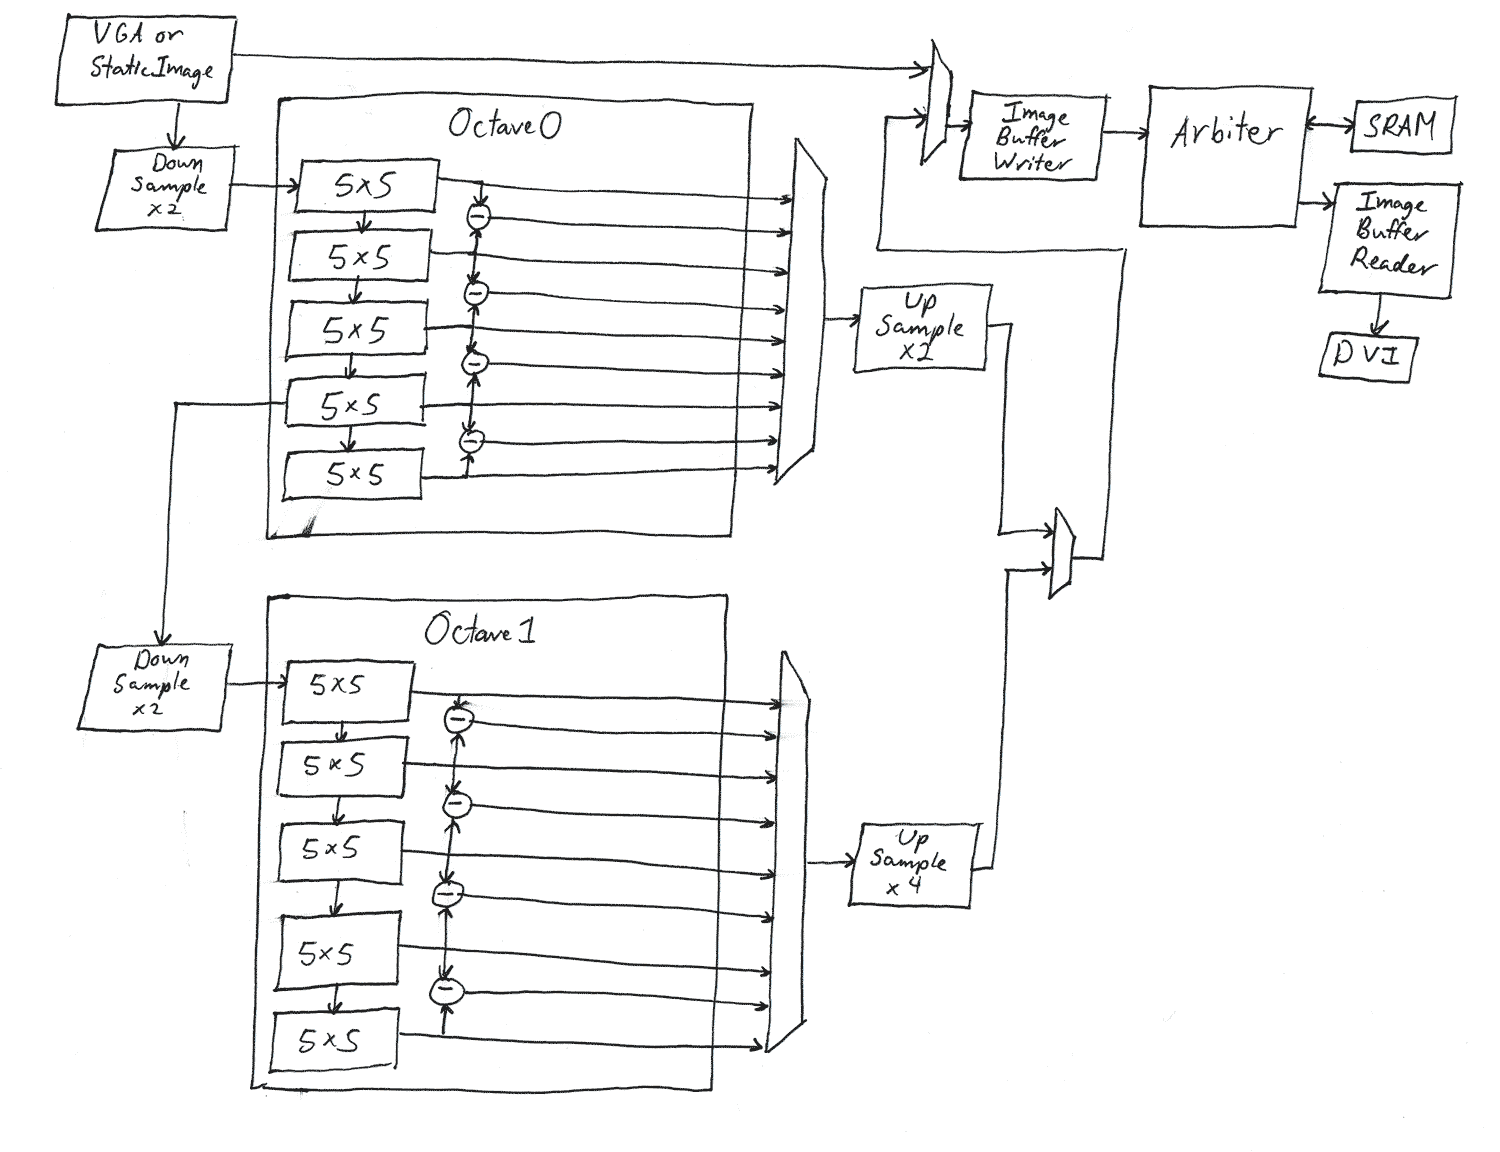
\includegraphics[width=0.7\textwidth]{processed_image_pngs/full_pipe_blackbox.png}
    \caption{Full-Pipeline Blackbox Image}
    \label{fig:full_pipe}
\end{figure}

See Figure \ref{fig:full_pipe}.


\subsection{Brief Description of Major Submodules}

\subsubsection{SRAM Arbiter}

The SRAM arbiter is the main interface between SRAM and the rest of our system.
Essentially, its task is to mediate reads and writes between other modules that
are competeting for access to our single port SRAM. The arbiter supports two 
write ports, two read ports, and services a single request (either a single 
read or a single write) per clock cycle.
SRAM\_arbiter\_blackbox.png

\subsubsection{Check4.v, Check4\_4x.v}

\begin{figure}
    \centering
    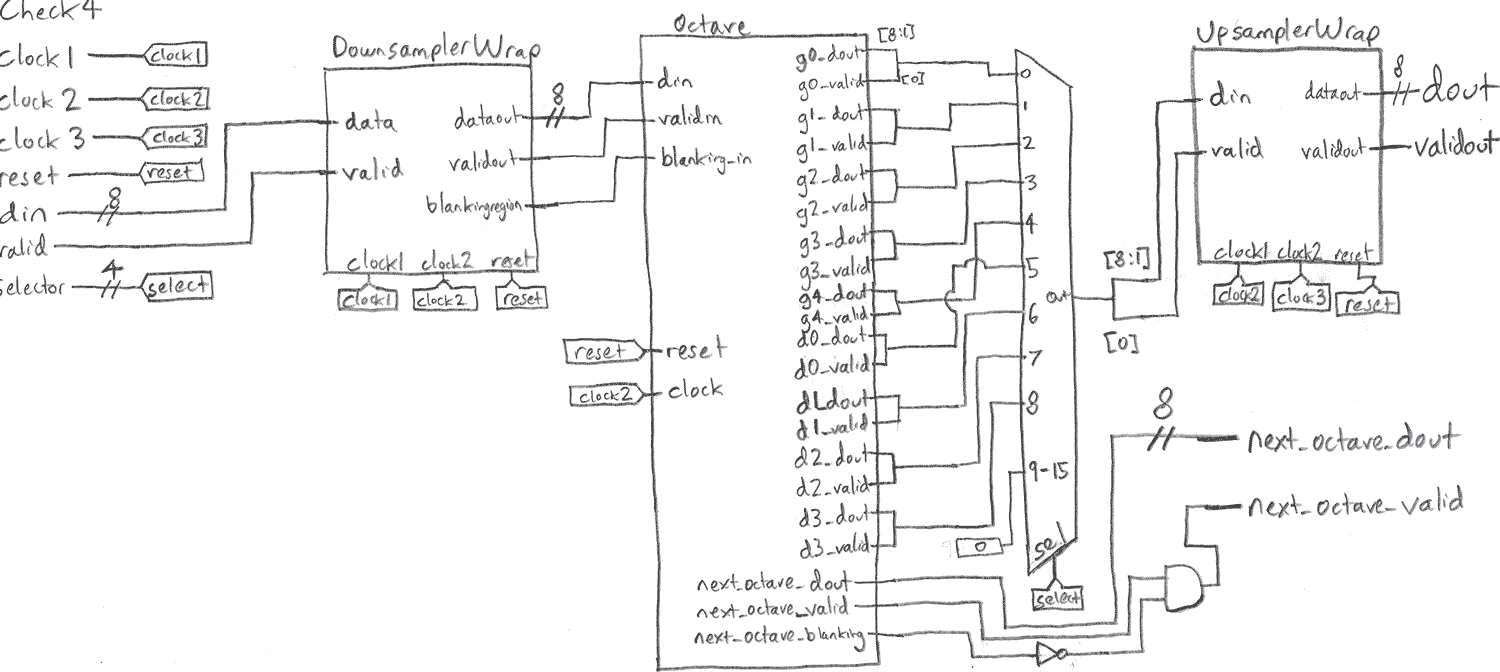
\includegraphics[width=0.7\textwidth]{processed_image_pngs/Check4.png}
    \caption{Check4.v Block Diagram}
    \label{fig:check_4}
\end{figure}

This module connects the entire Downsampler, Octave, and Upsampler pipeline together.
Additionally, it provides the switching functionality that allows our design to 
display any of the gaussians or differences on-demand. See Figure \ref{fig:check_4} for 
a detailed connection diagram.

\subsubsection{DownsamplerWrap.v, Downsampler4xWrap.v}

\begin{figure}
    \centering
    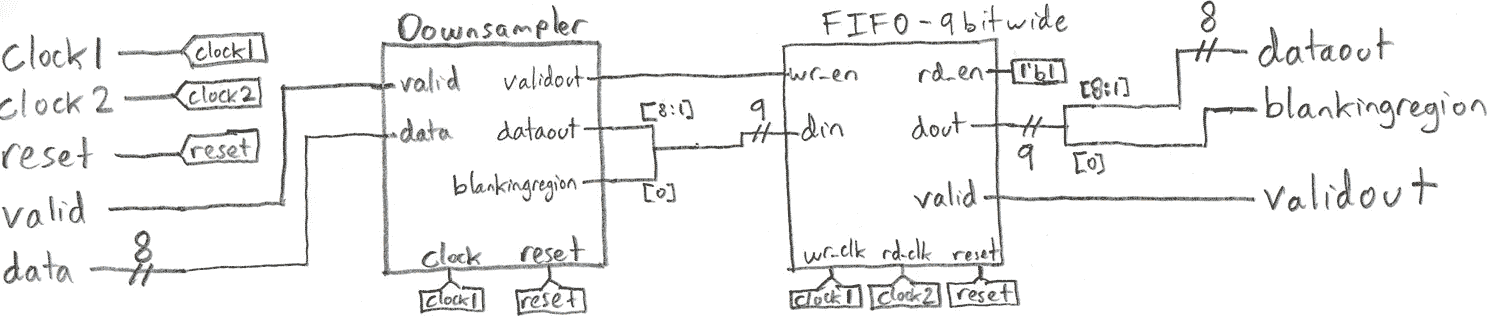
\includegraphics[width=0.7\textwidth]{processed_image_pngs/DownsamplerWrap.png}
    \caption{DownsamplerWrap.v Block Diagram}
    \label{fig:down_wrap}
\end{figure}


This module attaches the Downsampler to its output fifo, which mediates between
the Downsampler and the gaussian pipeline. This module spans both the first
and second clock domains. A detailed block diagram can be found in Figure \ref{fig:down_wrap}.

\subsubsection{UpsamplerWrap.v, Upsampler4xWrap.v}

\begin{figure}
    \centering
    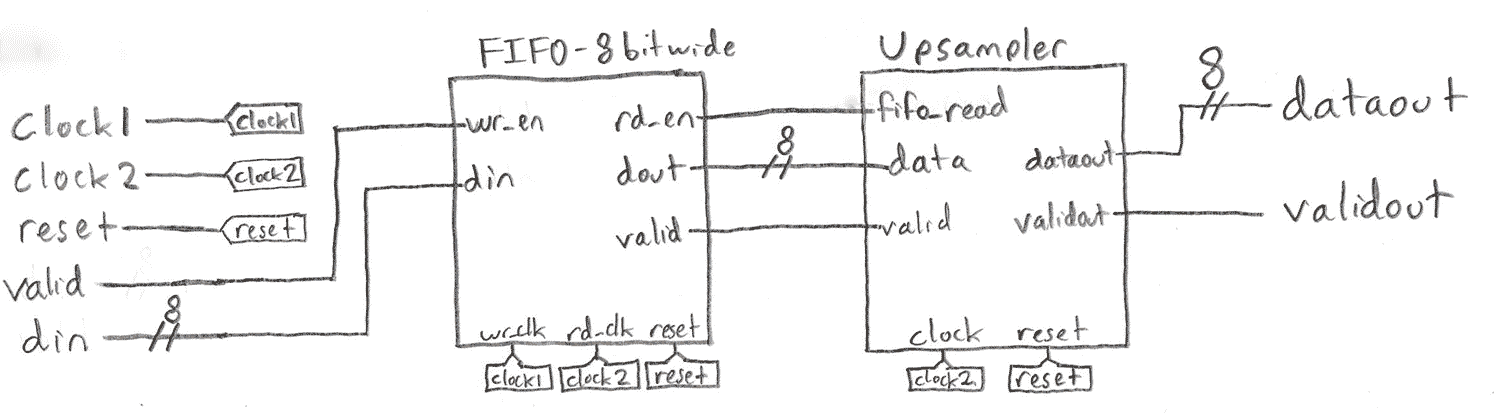
\includegraphics[width=0.7\textwidth]{processed_image_pngs/UpsamplerWrap.png}
    \caption{UpsamplerWrap.v Block Diagram}
    \label{fig:up_wrap}
\end{figure}


This module attaches the Upsampler to its input fifo, which mediates between
the gaussian pipeline and the Upsampler. This module spans both the second and
third clock domains. A detailed block diagram can be found in Figure \ref{fig:up_wrap}.

\subsubsection{Downsampler.v, Downsampler4x.v}

The Downsampler module converts the original 800x600 image fed into our processing
pipeline into a 400x300 image to align with our hardware constraints. The downsampler
takes in the image data as a stream of pixels along with a valid signal that is
only raised when the input pixel is valid data from the image. In addition to 
reducing image size, the downsampler is responsible for ``generating'' the 
blanking regions (sequences of black pixels) that are used to flush data 
through our gaussian pipeline. The downsampler ultimately outputs a scaled 
image as a stream of pixels along with a valid signal and a blankingregion 
signal that indicate whether the current output pixel is valid and/or a pixel
in the blanking region respectively. Downsampler4x.v is identical to 
Downsampler.v, excluding some constants that are modified to allow this version 
to downsample from 400x300 images to 200x150 images. A black-box diagram of the Downsampler
can be found in Figure \ref{fig:down_wrap}.

\subsubsection{Upsampler.v, Upsampler4x.v}

The Upsampler module converts the processed 400x300 image coming out of the processing
pipeline back into a 800x600 image for display over the DVI interface. The upsampler
takes in the processed image data as a stream of pixels along with a valid signal 
that is asserted only for data that is both valid pixel data from the image and
not part of the blanking regions. It performs basic upscaling by effectively taking
each pixel from the processed input and expanding it to cover a 2x2 box of 
pixels in the final output. The upsampler outputs a pixel at a time in the output 
image along with a validout signal that is asserted whenever the data on the 
output is valid pixel data that we ultimately wish to display (blanking regions
are non-existant at this point). Upsampler4x.v is identical to Upsampler.v, 
excluding some constants that are modified to allow this version to upsample 
from 200x150 images to 800x600 images. A black-box diagram of the Upsampler
can be found in Figure \ref{fig:up_wrap}.


\subsubsection{octave.v}

The Octave module contains 5 Gaussian filter blocks and computes the four 
Difference of Gaussian outputs. The module takes in a stream of pixels (one at 
a time), along with a valid signal and a blanking signal. It will output a 
stream of pixels (along with a valid signal) for each Gaussian filter and each 
Difference of Gaussian. There is no blanking output since blanking pixels are 
considered invalid at the output. This module also has a special output just 
for the next octave, which contains the data, valid, and blanking signal from 
one of the Gaussian filters (the fourth one in this case). A black-box diagram
of the Octave module can be found in Figure \ref{fig:check_4}.

\subsubsection{five\_by\_five\_window.v}

This module represents one Gaussian filter block, with five coefficients in the 
horizontal direction and five coefficients in the vertical direction. The input 
is a stream of pixels (one at a time), along with a valid signal and a blanking 
signal. The output is also a stream of pixels (after going through the Gaussian 
filter), along with a valid signal and a blanking signal. Pixels that are 
marked as blanking are also replaced with zero prior to the output. A black-box
diagram of the five by five window can be found in Figure \ref{fig:octave}.

\subsubsection{x\_window.v}

This module is used to compute the horizontal portion of the Gaussian filter. 
It will multiply 5 pixels in the same row by their corresponding coefficients. 
It will then take the average of those results to find the output value, whose 
location within the frame corresponds to the center of those five pixels. The 
input is a stream of pixels (one at a time), along with a valid signal and a 
blanking signal. The output is also a stream of pixels (after computing the 
horizontal Gaussian), along with a valid signal and a blanking signal. See Figure \ref{fig:five_window} for a 
black-box diagram.

\subsubsection{five\_row\_array.v}

This module is used to store five rows of pixels at a time, which becomes the 
input into the y\_window module. This module takes in a stream of input pixels 
(one at a time), along with a valid signal and a blanking signal. It outputs 
five pixels at a time, one from each line, along with a valid signal and a 
blanking signal. These five pixels have the same horizontal position in the 
frame, and come from consecutive lines within the frame. The center of these 
five consecutive lines is the pixel at the center of the Gaussian filter block, 
so the blanking output corresponds to the blanking input for this particular 
pixel. See Figure \ref{fig:five_window} for a 
black-box diagram.


\subsubsection{y\_window.v}

This module computes the vertical portion of the Gaussian filter. It multiplies 
5 input pixels (from the same column) by their corresponding coefficients, and 
averages those results to find the output value. The location of the output 
value within the frame corresponds to the center of the input pixels. The input 
is a stream of pixels (five at a time), along with a valid signal and blanking 
signal. The output is also a stream of pixels (after computing the vertical 
Gaussian), along with a valid signal and a blanking signal. See Figure \ref{fig:five_window} for a 
black-box diagram.


\section{System Description}

\subsection{Datapath}

\subsubsection{Connections to SRAM}

% [todo] - connections to SRAM
All interfacing with the SRAM in our design is done solely through the SRAM 
Arbiter designed in Checkpoint 2. This Arbiter follows the following state
transition rules when determining order-of-service for the two write and two read
ports. For this module, a state-diagram is prohibitive since it simply consists
of a complete graph over the 5 states (every possible transition exists). The 
five states that the SRAM arbiter can enter are PAUSE and the servicing states 
DOW0, DOW1, DOR0, and DOR1. Excluding the PAUSE state (which simply indicates 
that there are no requests being
processed), state names can be decoded in the following manner: the last two characters
stand for the port that is being serviced while the arbiter is in that state.
If we order the servicing states as they are presented above, we can see the priority given
to state transitions in our FSM. For example, if we are currently in state DOW1,
we will service the R0 port if a read requests exists there, the R1 port if a 
read requests exists there and not at R0, the W0 port if neither R0 or R1 have 
a request and W0 does and finally the W1 port again if there a request exists
and no other ports have a request. In any of our servicing states, if none of 
the ports have pending requests, we enter the PAUSE state, which follows the
same priority as the W1 state would. In this way, we maintain fairness of 
access to the SRAM, allowing different parts of our pipeline to interact
with the SRAM throughout execution.

\subsubsection{Difference of Gaussian Filter Blocks}

\begin{figure}
    \centering
    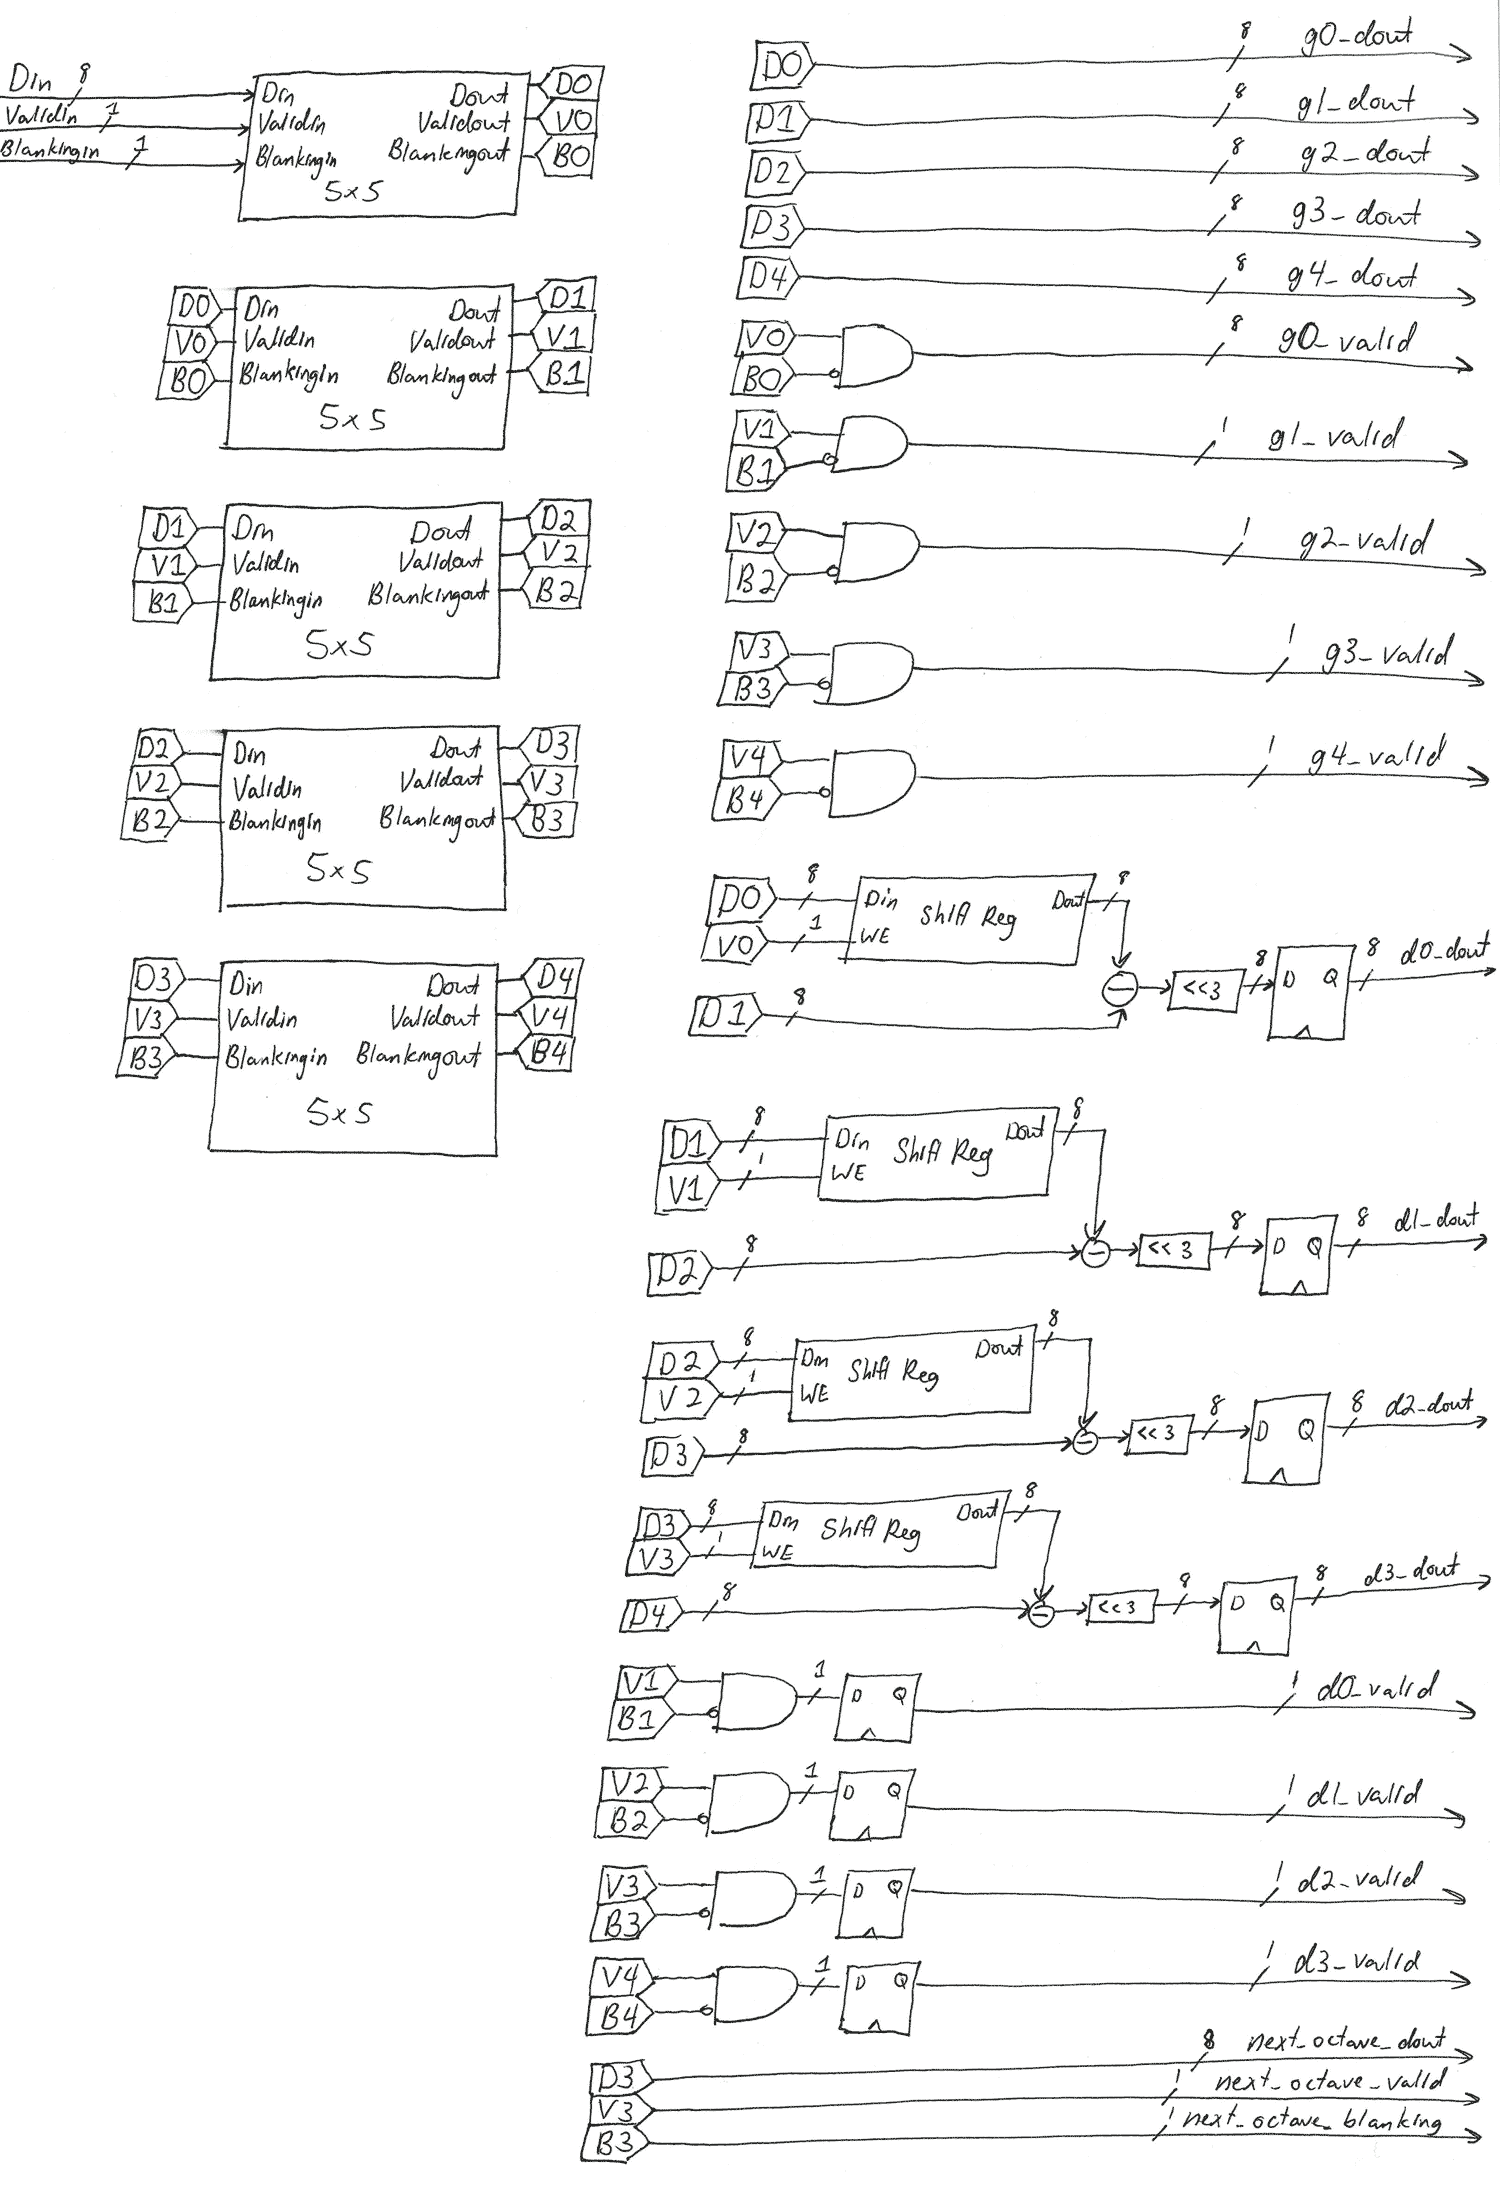
\includegraphics[width=0.9\textwidth]{processed_image_pngs/octave.png}
    \caption{Full Octave Block Diagram}
    \label{fig:octave}
\end{figure}

\paragraph{octave.v}

This module is where the each Difference of Gaussian is computed for a single octave. It contains five Gaussian filter blocks, where the output of one block is fed into the input of the next block. The time between the first valid pixel of one block and the first valid pixel of the next block is determined by the time it takes for one pixel to travel through an entire Gaussian filter. To compute a Difference of Gaussian, the same pixel from each Gaussian filter block needs to be used, despite the delay between the two blocks. This means that the output of the first Gaussian must be stored in a shift register with a depth equal to that delay, while also being routed to the next Gaussian filter block. The output of the next Gaussian is then subtracted from the output of the shift register. The result is the Difference of Gaussian. In order to make the Difference of Gaussian more visible, the result is also multiplied by eight (implemented as a left shift by three).

The blanking signal also needs to be delayed, however the second of the two 
Gaussians already takes care that, so the Difference of Gaussian simply uses the 
blanking signal of the latter Gaussian filter block. Blanking signals are used 
by other modules within the octave, and indicate whether or not a particular 
pixel is part of the original image (not blanking), or was added in order to pad 
the edges of the image (blanking). Blanking pixels are not used by any module 
outside of the octave, so blanking pixels are simply considered invalid pixels 
at the output.


\begin{figure}
    \centering
    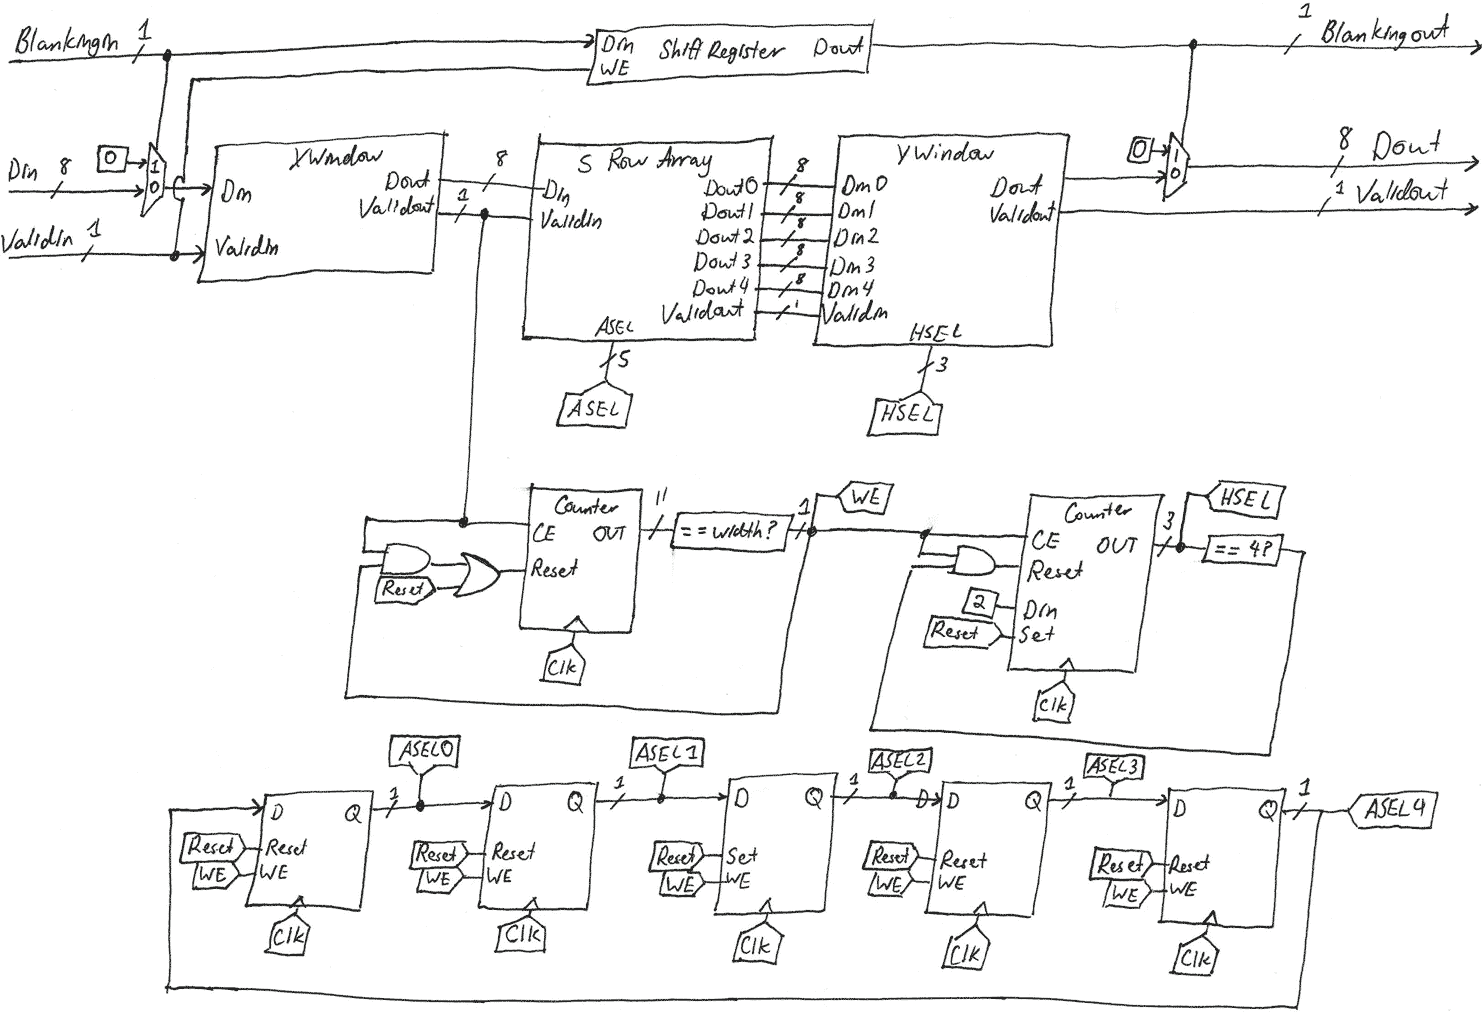
\includegraphics[width=0.7\textwidth]{processed_image_pngs/5x5_block.png}
    \caption{5x5 Window Block Diagram}
    \label{fig:five_window}
\end{figure}

\paragraph{five\_by\_five\_window.v}

This module is one Gaussian filter block. It is split into three sub-modules: 
x\_window, five\_row\_array, and y\_window. This module serves four main purposes:
1) To connect x\_window, five\_row\_array, and y\_window to each other and to the 
   inputs and outputs of the five\_by\_five\_window module
2) To generate control signals for five\_row\_array and y\_window
3) To delay the blanking input and ensure a proper blanking output
4) To replace any blanking input pixels and output pixels with zero
x\_window, five\_row\_array, and y\_window were designed so that they would connect 
directly to each other, in that particular order. The valid input into the 
module is fed straight into x\_window, and the valid output of y\_window is 
attached directly to the valid output of the five\_by\_five\_window.
The three sub-modules do not need the blanking input signal. This signal is 
instead put into a shift register, whose depth is equal to the delay it takes 
for one pixel to travel through x\_window, five\_row\_array, and y\_window. The 
output of this shift register is the blanking output signal.

The data into the five\_by\_five\_window module first goes into a mux, which 
chooses between the input data and a zero contestant, depending on if the input 
is part of a blanking region or not. The output of that mux is then fed directly 
into x\_window. In the same way, the output of y\_window goes into a mux, which 
chooses between the output data or a zero constant, depending on if the output 
is blanking. The output of this mux is connected to the data output of the 
five\_by\_five\_window module. This replacement of blanking pixels is done because 
those blanking pixels are used to pad the edges of the image, which is needed to 
keep the image size constant while feeding it through several Gaussian filters. 
In particular, the edges of the image need to be padded with zeros. However, 
running those zero pixels through an averaging filter will make them non-zero, 
which is why they need to be replaced by zeros between every filter block.
The control signals generated by this module for five\_row\_array and y\_window 
will be discussed in a later section.

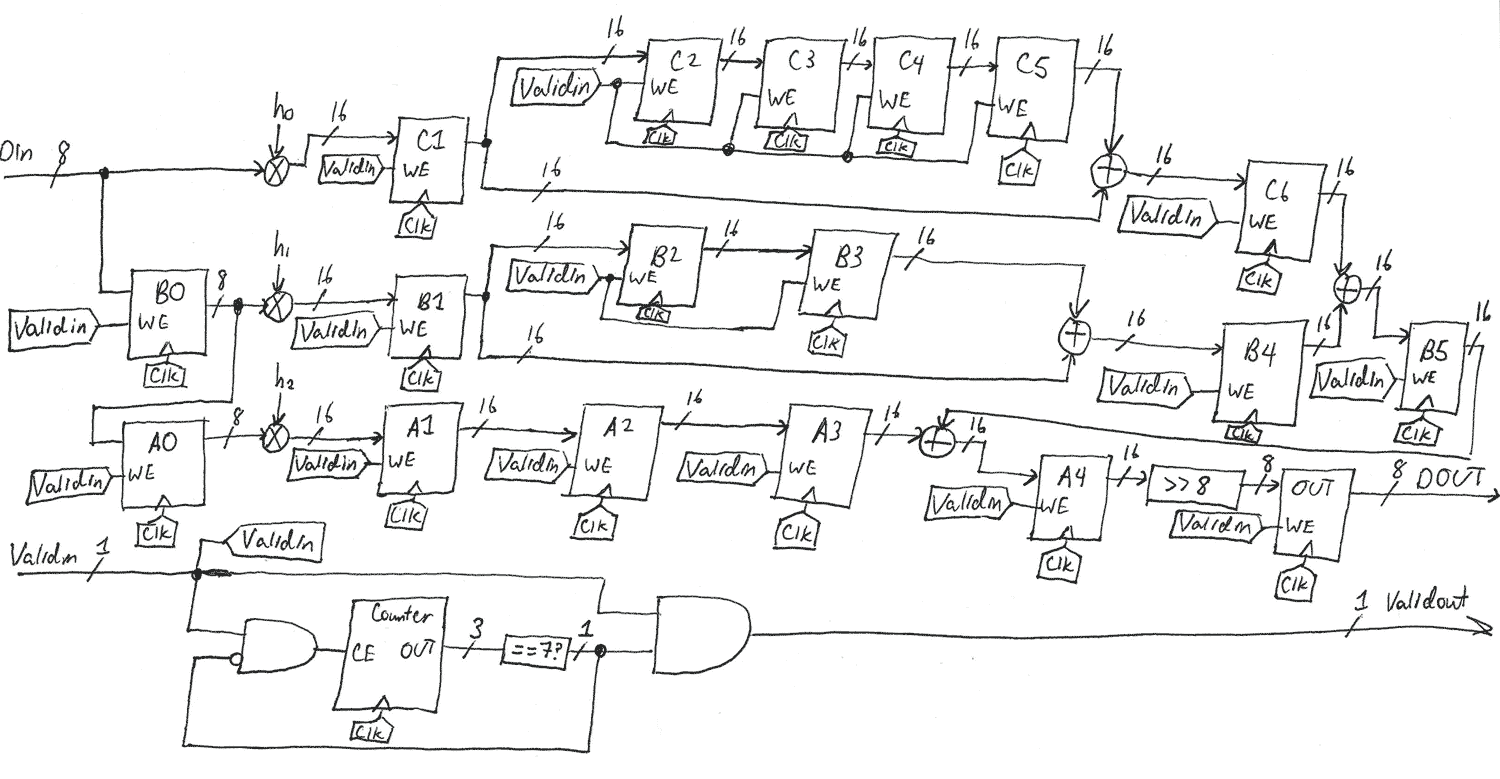
\includegraphics[width=\textwidth]{processed_image_pngs/x_window.png}

\paragraph{x\_window.v}

This module computes the horizontal portion of the Gaussian filter. The basic 
idea is that the module will store the 4 previous input pixels and the current 
pixel. It will also multiply each pixel by its coefficient, add the result of 
those operations, and scale the result back down to an 8-bit value for the next 
stage.

The module expects the value of each pixel in the frame as input, one line at 
a time (top to bottom), starting from the first (leftmost) pixel in the line and 
ending at the last (rightmost) pixel in the line. This module does not take into 
account padding. If the image is inputted without extra padding pixels, then the 
results at the edges of each line may not be accurate. To ensure proper results, 
there needs to be at least two blanking pixels at the end of this line (assuming 
the horizontal Gaussian window takes in five pixels). The two pixels can act as 
padding for both the previous line and the next line. An illustration of this 
concept is shown below:

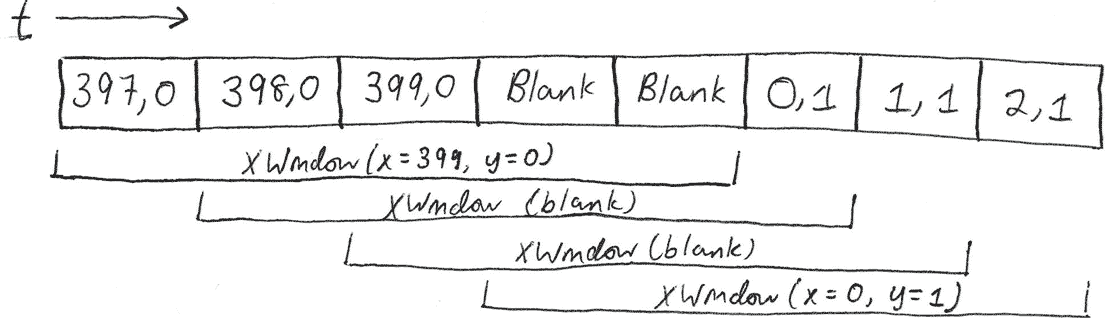
\includegraphics[width=\textwidth]{processed_image_pngs/serial_input.png}

Since all registers are set to 
zero upon reset, including the registers that store previous pixel values, the 
first two pixels of the frame are already padded.

In order to ensure maximum clock frequency, there is a register between each 
consecutive mathematical operation, such as a multiplication and addition. 
Because of this, computing the sum of all five terms takes several cycles, and 
adds some latency to this portion of the pipeline. However, once the pipeline is 
filled, there will be one valid output during every cycle with a valid input 
(invalid inputs will stall the pipeline). The time it takes to generate an 
output for a particular input (assuming the pipeline is not stalled after this 
point) is 7 cycles. This is also the time it takes to fill the pipeline. 
Therefore, there is a 7 cycle delay between when the valid input signal becomes 
high and when the valid output signal becomes high (again, assuming there are no 
stalls).

This module also takes advantage of the symmetry in the Gaussian coefficients, 
and computes the product of a pixel and its coefficient only once. For example, 
once the product of some pixel and the coefficient h1 is computed for the first 
time, that value will be needed again two cycles later. Likewise, the product of 
some pixel and the coefficient h0 will be needed 4 cycles later. The module will 
store and shift this value down the pipeline where it will be used for later 
operations which require this result. This reduces the number of multipliers in 
the module, which reduces the overall number of DSP SLICEs required for this 
particular module.

The coefficients are scaled in such a way that the result of adding each term 
(the product of a pixel and its coefficient) is no larger than a 16-bit unsigned 
number. In order to scale this back down to an 8-bit number, we simply keep the 
upper 8 bits and drop the lower 8. This is the same as dividing the result by 
256, or shifting the result to the right by 8.

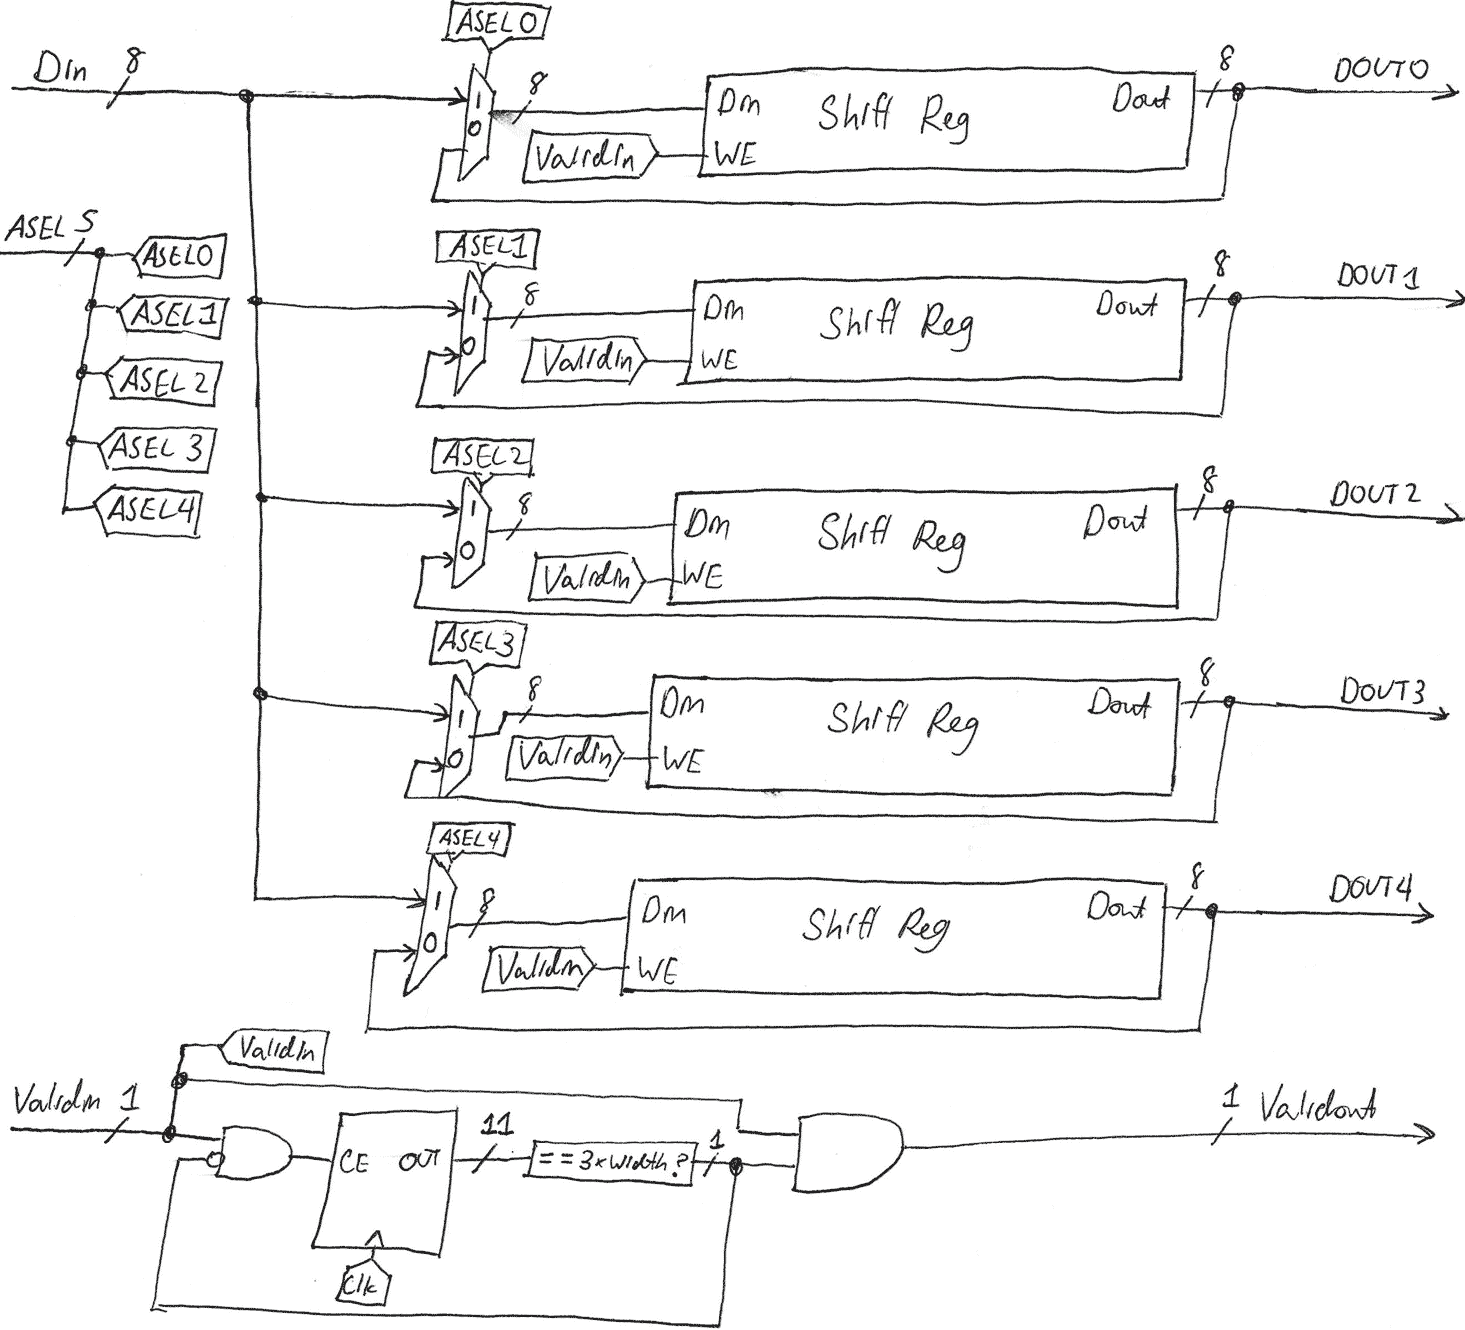
\includegraphics[width=0.75\textwidth]{processed_image_pngs/array.png}

\paragraph{five\_row\_array.v}
This module stores the results of the x\_window module. Each output of x\_window 
is the result of running each pixel through the horizontal portion of the 
Gaussian filter. This module will store 5 lines worth of pixels, which is needed 
to compute the vertical portion of the Gaussian filter. The output is five pixel 
values, all from the same position within a line (column), from five consecutive 
rows. This is accomplished by creating a 5 shift registers, one for each line, 
with a depth equal to the number of pixels in a line (including blanking).
The module is constantly shifting values in and out of each shift register, as 
long as there is a valid input. One of the five shift registers gets new values 
from the input, and every other shift register has its output fed back into the 
input. This is done to ensure that a pixel of a particular position within 
a line (such as x=250) is in the same position within all 5 shift registers. The 
array containing the oldest values gets replaced by newer values. Once that 
array is full, the module will begin filling/replacing the contents of the next 
oldest array. An illustration of this concept is shown below: 

%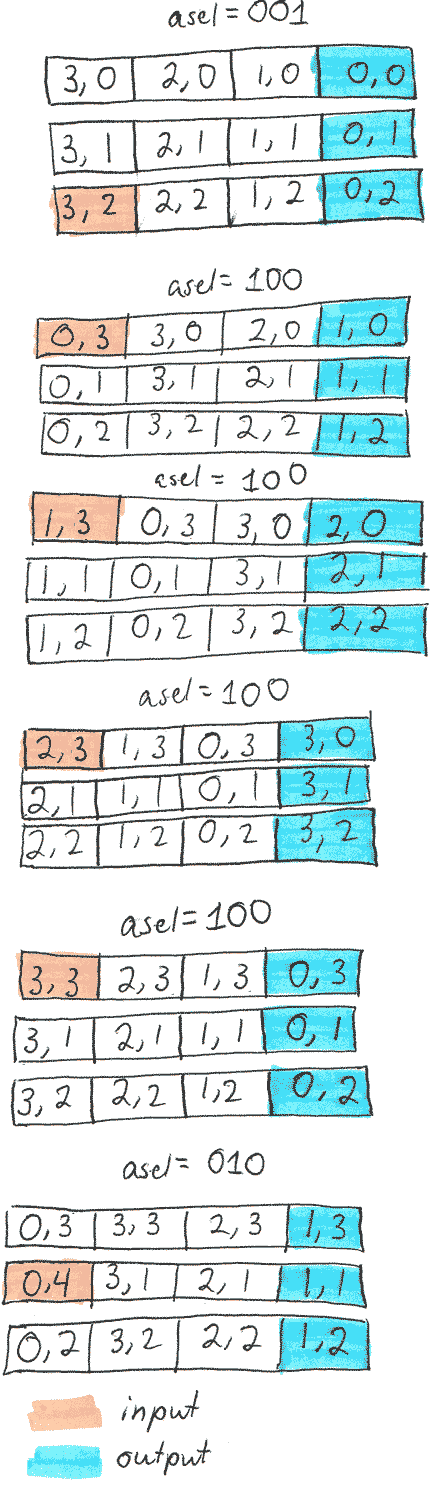
\includegraphics[width=\textwidth]{processed_image_pngs/io_diagram.png}
\begin{wrapfigure}{r}{0.25\textwidth}
    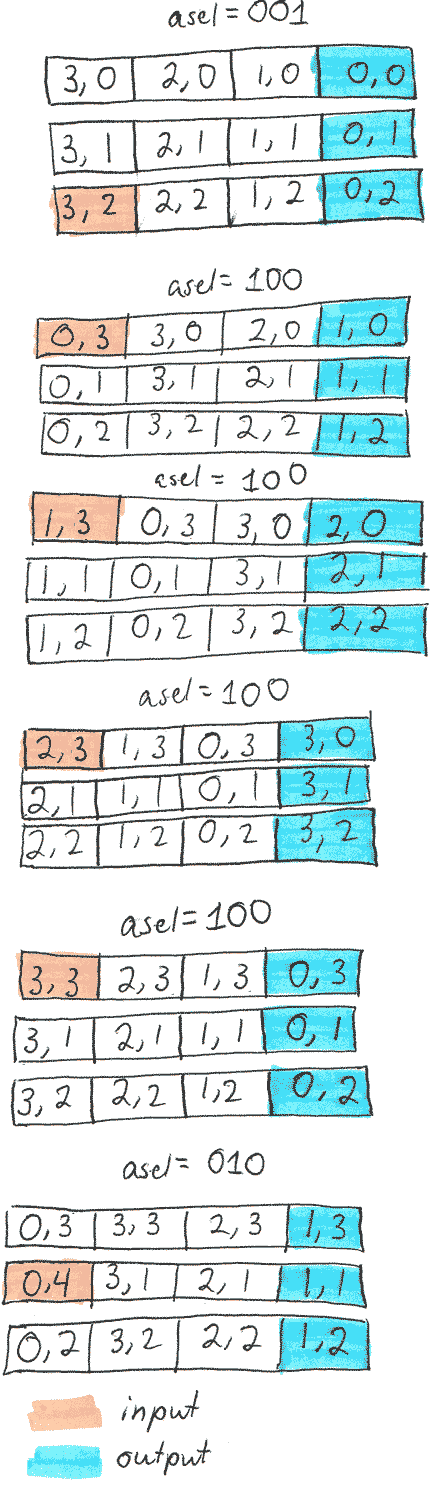
\includegraphics[width=0.23\textwidth]{processed_image_pngs/io_diagram.png}
\end{wrapfigure}


The input signal asel is used to choose which array to shift the new value into. 
This is a five-bit, one hot signal. Each bit corresponds to a particular 
shift register, and if that bit is 1 then the shift register will shift in the 
new data (instead of shifting in the old data). As long as each new value is 
shifted into the proper register in the proper order, then the outputs will also 
be in the proper order. See the example above for a demonstration on how this is 
accomplished.

Only the first three rows need to be filled before there is a valid output. This 
is because the shift registers are set to 0 upon reset, so two of the rows can 
act as blanking rows. This means that the delay between a valid input and 
a valid output (assuming no stalls/invalid inputs) is 3*width, where width is 
the number of pixels in a row, including blanking. This is also the time it 
takes to fill this portion of the pipeline, and the time it takes to generate an 
output for one particular input.

Note that the first shift register does not always correspond to the first line 
within the vertical Gaussian window (nor does the second shift register 
correspond to the second line, and so on). This is because the current line 
being filled with new data is always rotating (according to the input asel). 
This means that the y\_window module needs to keep track of which line is which, 
and select the appropriate coefficients for each line. How and where these 
control signals are generated will be discussed in a later section.


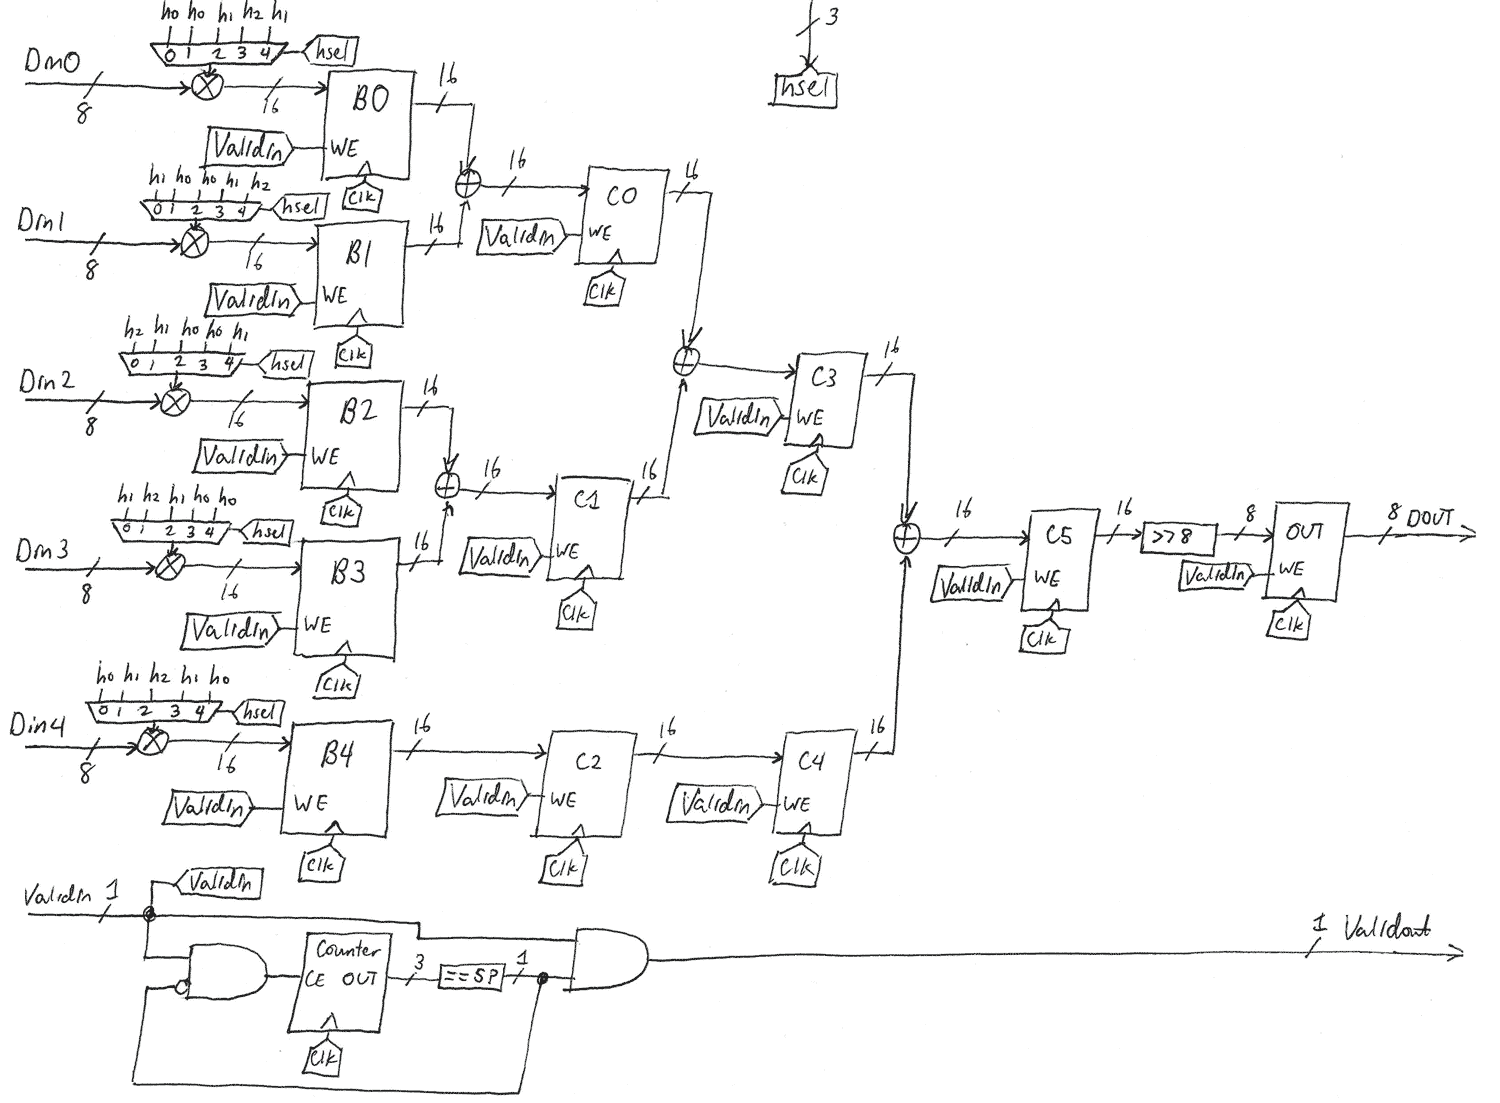
\includegraphics[width=0.8\textwidth]{processed_image_pngs/y_window.png}

\paragraph{y\_window.v} 

This module computes the vertical portion of the Gaussian filter. It 
will receive five input pixels from the five\_row\_array. Each pixel is from the 
same position in a line (such as x=250), and comes from consecutive lines. It is 
expected that the pixels will start from the leftmost position within a line, 
and end at the rightmost position. It is also expected that the groups of lines 
will be received in order from top to bottom (i.e. lines \lbrack 1,2,3,4,5 \rbrack followed by 
lines \lbrack 2,3,4,5,6 \rbrack). These pixels are then multiplied by their corresponding 
coefficients and the results are added together. This sum will then be scaled 
back down to an 8-bit number. To ensure proper results, at least two extra lines 
of zeros (blanking/padding), need to be added at the end of each frame. This is 
similar to the requirement of two extra pixels in each line for the x\_window 
module.

In order to ensure maximum clock frequency, there is a register between each 
consecutive mathematical operation, such as a multiplication and addition. 
Because of this, computing the sum of all five terms takes several cycles, and 
adds some latency to this portion of the pipeline. However, once the pipeline is 
filled, there will be one valid output during every cycle with a valid input 
(invalid inputs will stall the pipeline). The time it takes to generate an 
output for a particular input (assuming the pipeline is not stalled after this 
point) is 5 cycles. This is also the time it takes to fill the pipeline. 
Therefore, there is a 5 cycle delay between when the valid input signal becomes 
high and when the valid output signal becomes high (again, assuming there are no 
stalls). This is shorter than the 7 cycle delay of the x\_window module because 
this module receives all 5 pixels at once, rather than having to store each 
pixel one at a time until there is enough for a valid output.

As we pointed out in the previous section, the outputs of the five\_row\_array do 
not always correspond to the same line within the vertical Gaussian window. This 
means that the inputs to y\_window, which are connected directly to the outputs 
of five\_row\_array, also do not correspond to the same line. This also means that 
the coefficients (that we multiply each input by), cannot be constant. The 
signal hsel, which is a 3-bit number ranging between zero and four, is used to 
choose the coefficient for each line. In terms of hardware, this means that 
there is a 5-mux (for each line) which chooses between the five coefficients, 
and the result is then fed into the multiplier (for each line). The same signal 
hsel is used for all five multiplexers. What is different is the order in which 
the coefficients are attached to each multiplexer. This allows one signal, hsel, 
to choose between the 5 different ways in which the outputs from five\_row\_array 
can be arranged. As long as hsel and asel are in synch, and change at the same 
time, the proper coefficients will be used. Details on how hsel and asel are 
generated will be discussed in a later section.

The coefficients are scaled in such a way that the result of adding each term 
(the product of a pixel and its coefficient) is no larger than a 16-bit unsigned 
number. In order to scale this back down to an 8-bit number, we simply keep the 
upper 8 bits and drop the lower 8. This is the same as dividing the result by 
256, or shifting the result to the right by 8.


\subsubsection{Connections to ImageBufferWriter}

\begin{wraptable}{r}{5.5cm}

    % [todo] - transpose the table for space fix

    \begingroup
    \tiny
    \caption{ NOTE: Any missing binary numbers (switch combinations) are considered illegal 
and will cause the swap controller to stall.} \label{wrap-tab:1}
\begin{tabular}{ c | c | c } \toprule
Binary & Octave & Image\\\toprule
00000 & 0 & gauss0\\ \midrule
00001 & 0 & gauss1\\ \midrule
00010 & 0 & gauss2\\ \midrule
00011 & 0 & gauss3\\ \midrule
00100 & 0 & gauss4\\ \midrule
00101 & 0 & diff0\\  \midrule
00110 & 0 & diff1\\  \midrule
00111 & 0 & diff2\\  \midrule
01000 & 0 & diff3\\  \midrule
10000 & 1 & gauss0\\ \midrule
10001 & 1 & gauss1\\ \midrule
10010 & 1 & gauss2\\ \midrule
10011 & 1 & gauss3\\ \midrule
10100 & 1 & gauss4\\ \midrule
10101 & 1 & diff0\\  \midrule
10110 & 1 & diff1\\  \midrule
10111 & 1 & diff2\\  \midrule
11000 & 1 & diff3\\  \bottomrule
\end{tabular}
\endgroup
\end{wraptable}


ImageBufferWriter only requires a data input and a valid signal, and this comes 
from the upsampler. In this case, we have two upsamplers, one from each octave. 
Each octave also has nine outputs: five Gaussian outputs and four Difference of 
Gaussian outputs. This means that we need to choose which one of those outputs 
goes into the upsampler, and then choose which upsampler to connect to 
ImageBufferWriter. The selector input for the Check4 and Check4\_4x modules is 
used to choose between the five Gaussian outputs and the four Difference of 
Gaussian outputs. The value of selector is determined by GPIO\_DIP[3:6]. Inside 
of FPGA\_TOP\_ML505, we use GPIO\_DIP[7] to choose which upsampler to connect to 
ImageBufferWriter. If we consider GPIO\_DIP[3:7] (a particular combination of 
switches) to be a 5-bit binary number, then the following table summarizes which 
image each number corresponds to:


Switching the input to ImageBufferWriter at the wrong time could result in 
a shifted image or a stalled swap controller. In order to mitigate these issues, 
the GPIO\_DIP switches are not connected directly to the selectors/multiplexors. 
Instead, these values are stored in a register and that register is updated at 
a time when it is safe to switch. The details of this implementation and the 
timing will be discussed in a later section.


\subsubsection{Downsampler}

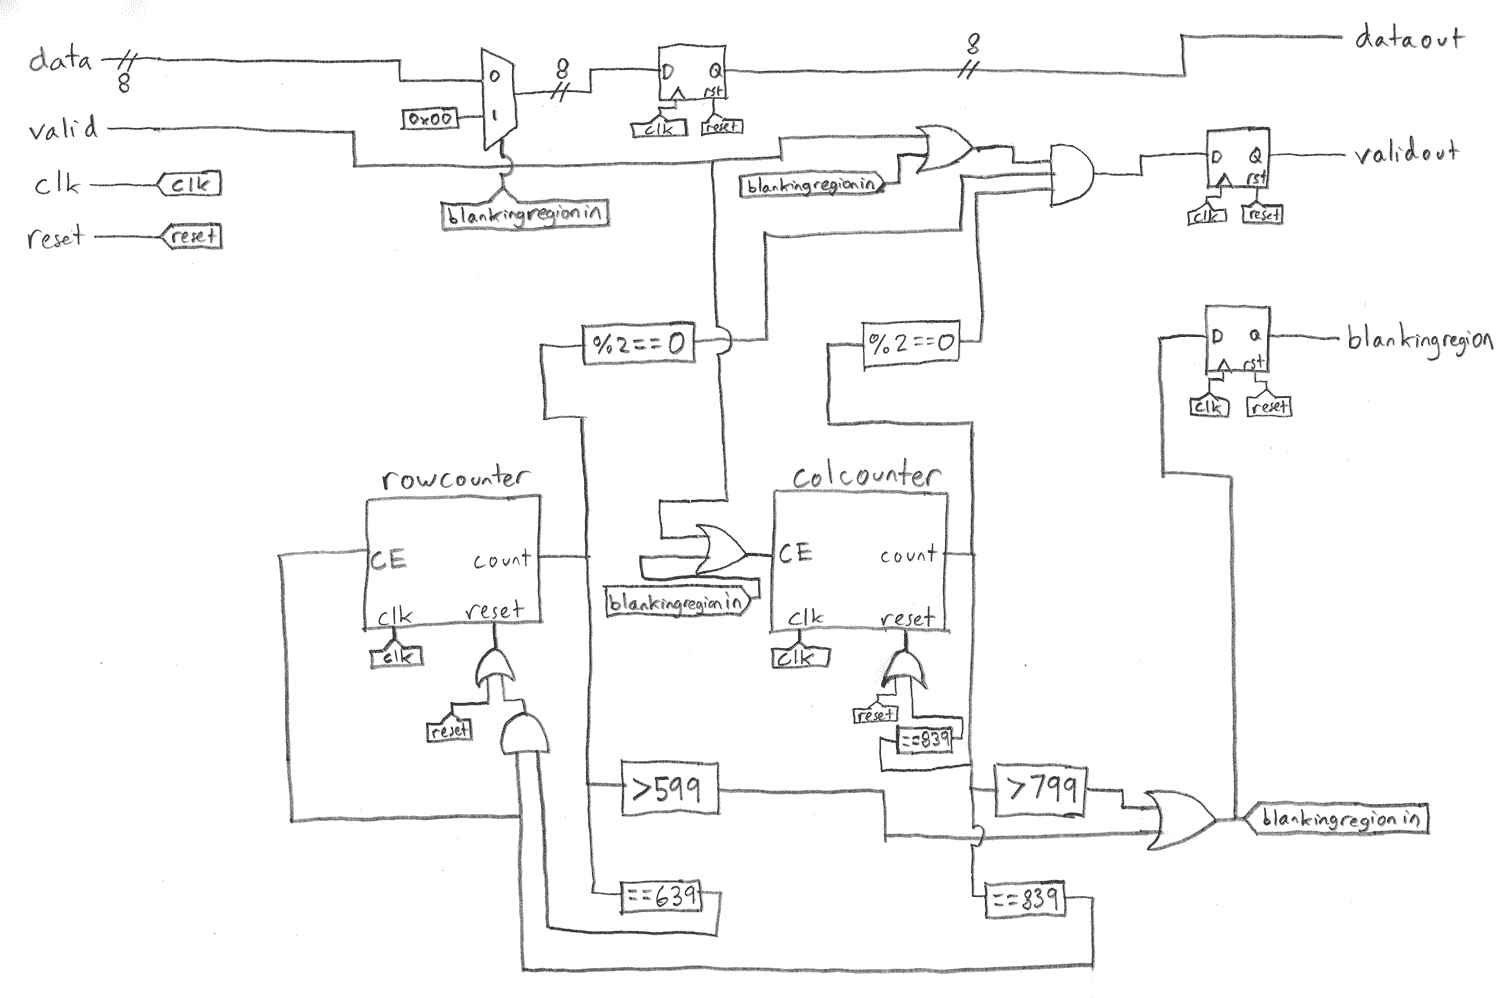
\includegraphics[width=\textwidth]{processed_image_pngs/Downsampler.png}

This module achieves two main data pre-processing goals for our system. Firstly,
it scales the input image from 800x600 pixels per frame to 400x300 pixels per frame.
Additionally, it provides ``stable'' blanking region generation in order to 
flush valid data from our pipeline at the end of a line and the end of a frame.
In doing so, it allows our pipeline to accept any input image that does not 
produce a valid output for at least 40 cycles at the end of a line and 40 lines
at the end of a frame. These are reasonable values since they are far lower than
the blanking regions generated by the VGA interface. The main feature in the
datapath of the downsampler is a set of 3 registers, each tied to one of 
dataout (the 8 bit pixel output), validout (a 1-bit signal that is asserted if
the output data is either part of the output image or part of a blanking region), 
and blankingregion (a 1 bit-signal that is asserted when the dataout value is
a blanking region). The values fed into these registers are computed using 
the output of a set of two counters, which we will discuss in detail in section 
% [todo] - add section number in downsampler section
. Essentially, the validout signal is asserted for 420 cycles for every other row 
of the original image, plus 20 additional rows for blanking. The blankingout signal
is similarly asserted for 20 cycles at the end of a row of the image and for
20 rows at the end of a frame of the image. This produces a 420x320 input image
for the rest of the pipeline to process.

\subsubsection{Upsampler}

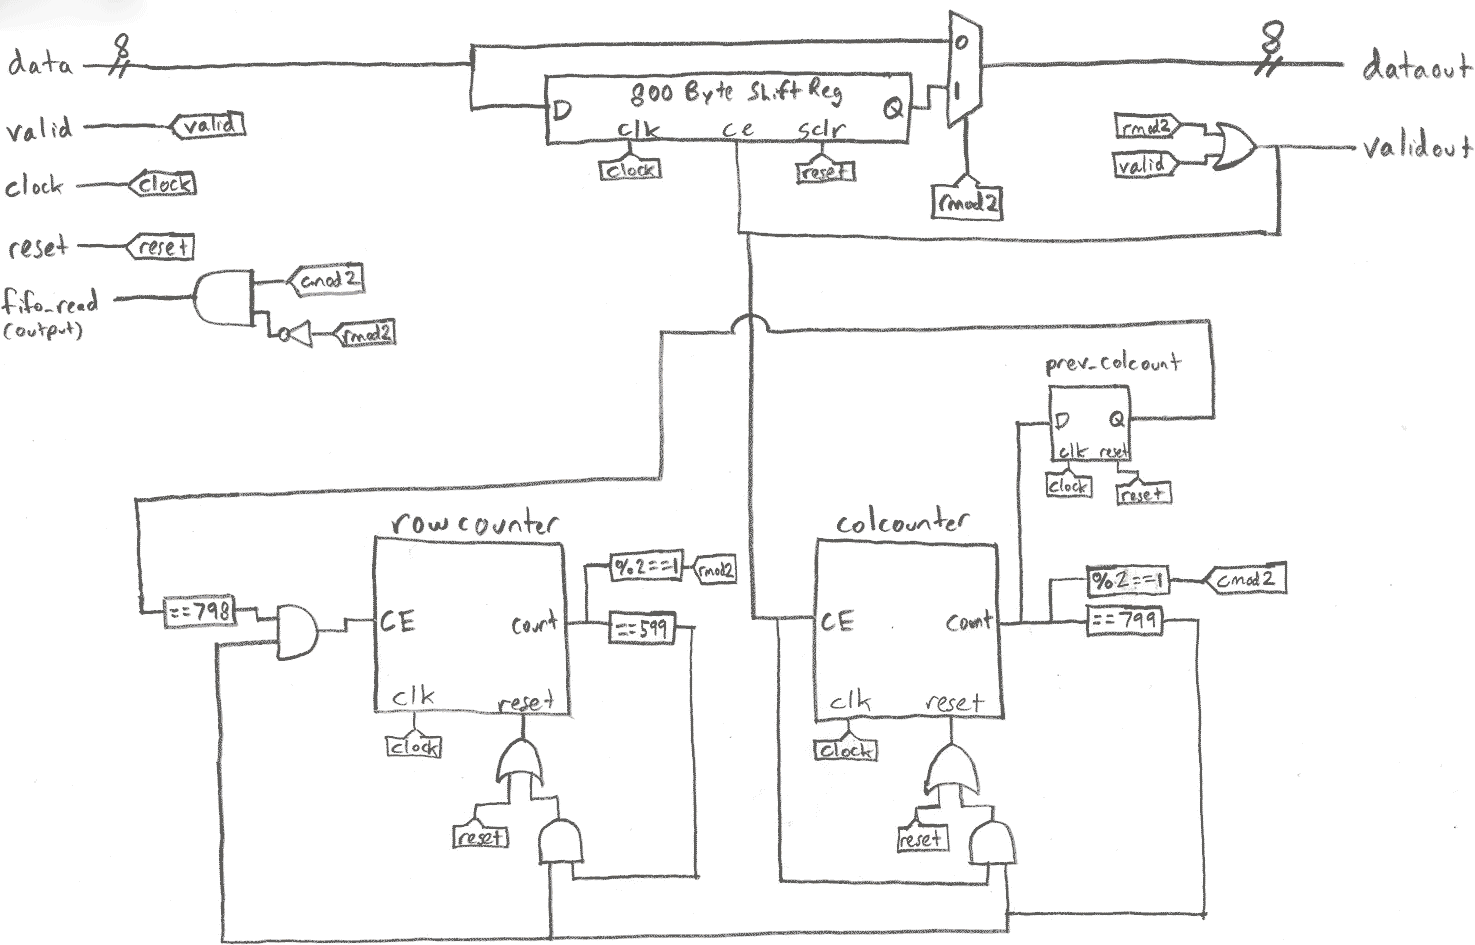
\includegraphics[width=\textwidth]{processed_image_pngs/Upsampler.png}

This module takes our processed 400x300 images and scales them up by 2x in each
direction to produce an 800x600 image. The upsampler duplicates pixels using 
two methods. First, to duplicate in the horizontal direction, we simply instruct
the fifo from which we are reading data to maintain each valid output on its
data output line for exactly two cycles. Because we are utilizing the 
first-word-fall-through functionality of the FIFOs, we do not need to explicitly 
assert read enable in order to ``get'' values. Rather, the next value that the
fifo is able to present is simply held at its output until we request the ``next'' value.
Thus, upon seeing the assertion of the valid signal of the upsampler fifo, we simply
wait one clock cycle before asserting our read enable signal to ``clear out'' the old
value. Thus, as far as our output is concerned, we receive two copies of each valid
pixel in the horizontal direction. Additionally, to produce the 2x duplication
in the vertical direction, we take the output from our horizontal duplication ``stage''
and feed it into a shift register that is 800 bytes wide. Thus, once we have
processed an entire valid row of 400 input pixels (which outputs 800 valid pixels and 
additionally fills the shift register with 800 valid pixels), we switch our modules 
output to the output of the shift register and run for 800 cycles. This produces
the duplicate row that we need for vertical scaling. This entire mechanism is
controlled by a set of counters, which will be discussed in the control section.

\subsection{Control}

\subsubsection{Dealing with issues - blank rows, addressing issues}

\subsubsection{General controller design, by module}

\paragraph{octave.v}
This module does not need any control signals or generate any control signals. 
However, it does depend on an input signal validin, and outputs a valid signal 
for each Gaussian and Difference of Gaussian. If there is no valid input, then 
the entire pipeline is stalled, and there are no valid outputs. When there are 
valid inputs, and the pipeline is still filling up, some Gaussian filter blocks 
will have a valid output and some will not. This is because the output of one 
Gaussian filter is fed into the input of the next Gaussian. This also means that 
the same pixel (for example, the first pixel), will be outputted at different 
times for different Gaussians. Once the entire pipeline has been filled, all 
outputs will be valid as long as there is a valid input as well. However, there 
is still a delay between the time when a particular pixel (i.e. a pixel at one 
specific location within the frame) shows up on the output of each Gaussian 
filter block. This delay is just the delay through all of the components of the 
Gaussian filter block (x\_window, five\_row\_array, and y\_window). The total delay 
is then (3*width)+12, where width is the number of pixels in one line, including 
blanking. Suppose width = 420, and the octave receives a constant stream of 
valid outputs starting at cycle 0. Then:

g0\_valid = 1 @ cycle 1272
g1\_valid = 1 @ cycle 2544
d0\_valid = 1 @ cycle 2545
g2\_valid = 1 @ cycle 3816
d1\_valid = 1 @ cycle 3817
g3\_valid = 1 @ cycle 5088
d2\_valid = 1 @ cycle 5089
g4\_valid = 1 @ cycle 6360
d3\_valid = 1 @ cycle 6361

Note that the output for each Difference of Gaussian is delayed by one extra cycle. This is because there is a register after the subtraction and right shift operations to pipeline the output. Any stall in the pipeline (i.e. an invalid input into the octave for n number of cycles) will cause an additional delay.

\paragraph{five\_by\_five\_window.v}
This module does not need any control signals. However, it does generate the 
control signals asel and hsel for five\_row\_array and y\_window, respectively. 
These signals are only supposed to change when the x\_window module outputs 
enough pixels for one complete line. This was done by making a counter, which 
goes from 0 to width-1 (where width is the number of pixels in one line, 
including blanking), and increments when there is a valid output from x\_window. 
The state machines which generate asel and hsel will change states whenever the 
counter is equal to width-1. Both state machines are Moore machines which simply 
rotate between five different states. These states correspond to the five 
different ways in which the outputs of five\_row\_array can be arranged. The state 
diagrams for these machines are below:


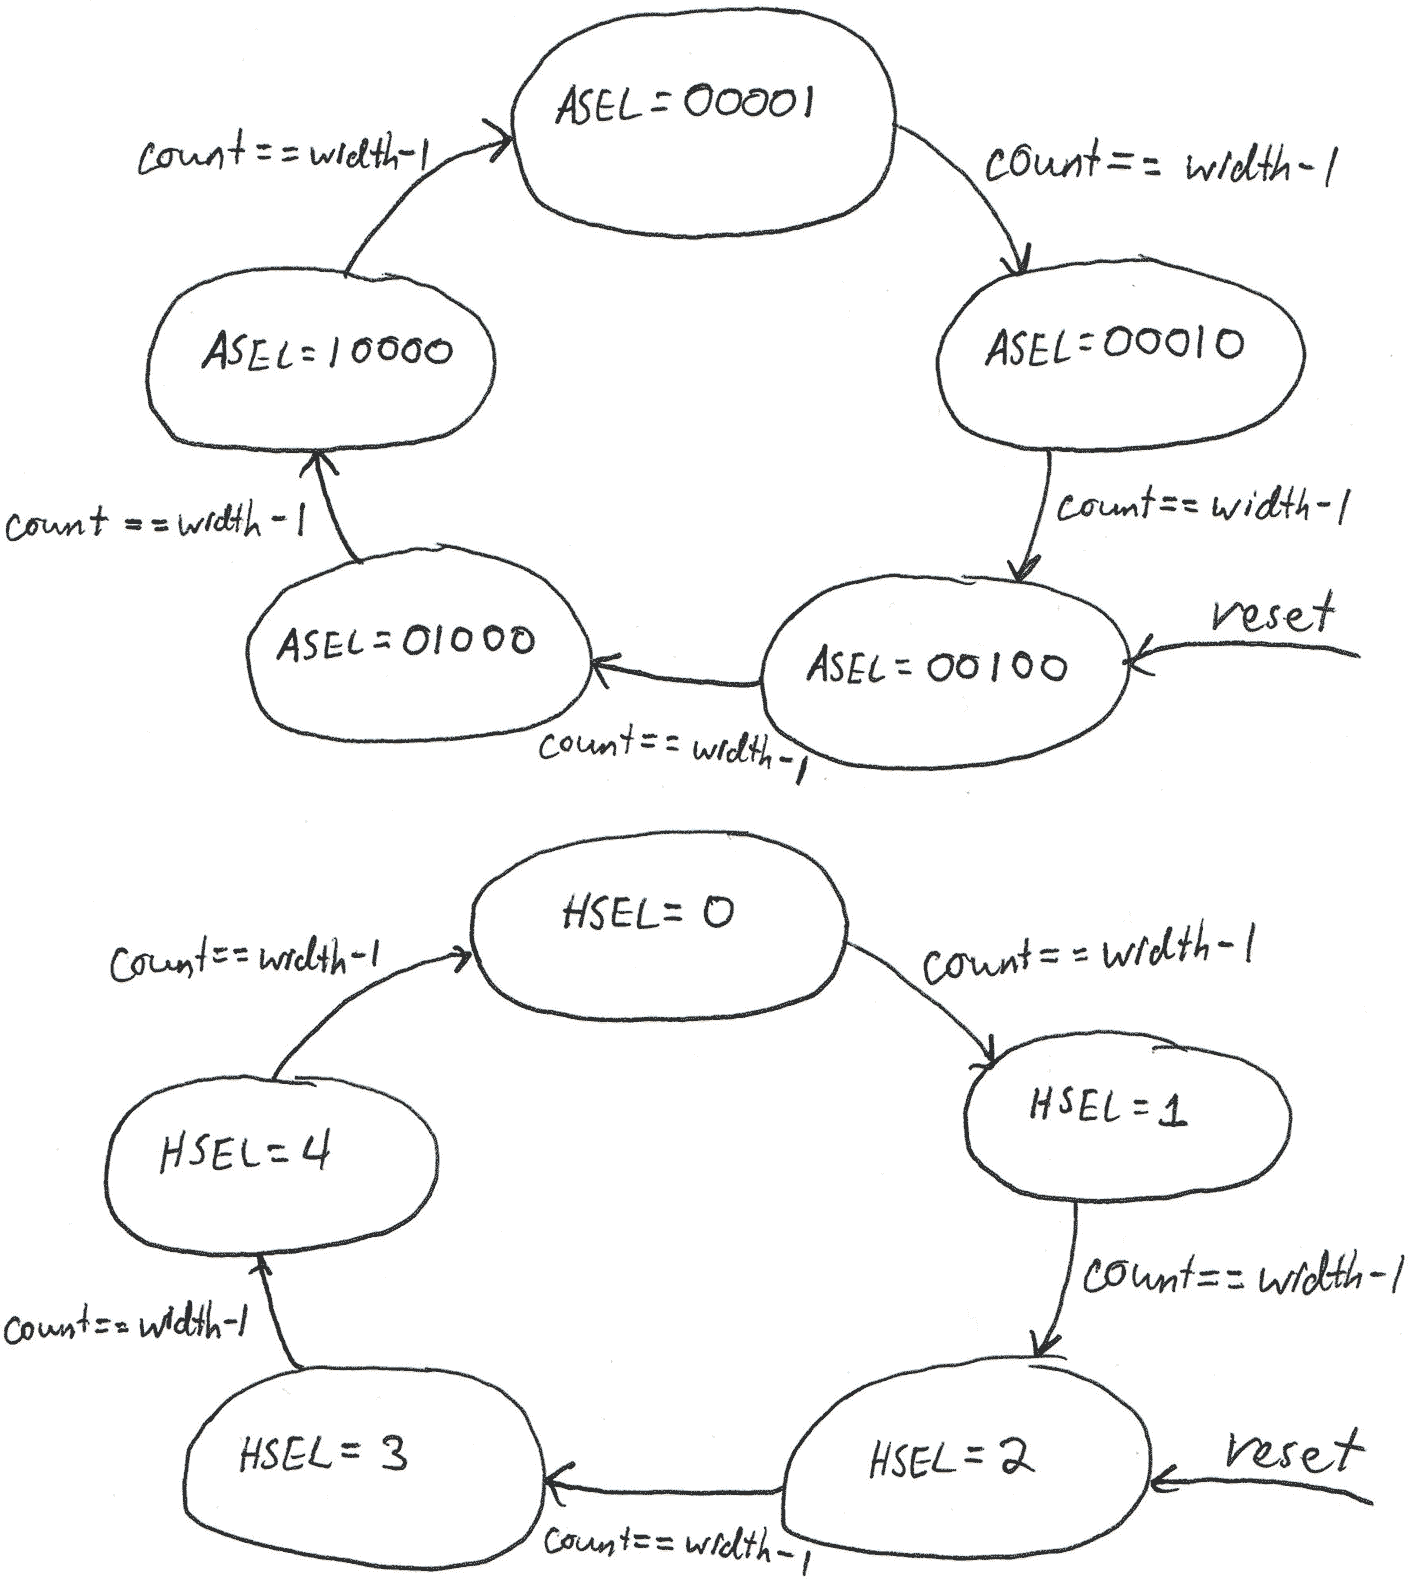
\includegraphics[width=0.75\textwidth]{processed_image_pngs/sel_states.png}


This module also takes in a valid signal and outputs a valid signal. However, 
this modules does not do anything to these signals; it simply feeds the input 
into x\_window, and takes the output directly from y\_window. The behavior of this 
module's sub-modules (x\_window, five\_row\_array, and y\_window) does mean that 
this entire module will stall if there is no valid input.

\paragraph{x\_window.v}
This module does not need any control signals nor does it generate any control 
signals. It does have a simple counter to determine if the pipeline has filled 
up enough so that the output is valid. This counter will increment as long as 
there is a valid input, and the count is less than seven. Once the count has 
reached seven, the counter will stop incrementing unless the module is reset. 
The output of the module is invalid if the counter is less than seven, or the 
input is not valid. This also means that an invalid input will stall this 
module. A timing diagram demonstrating the relationship between validin, the 
counter, and validout is below:

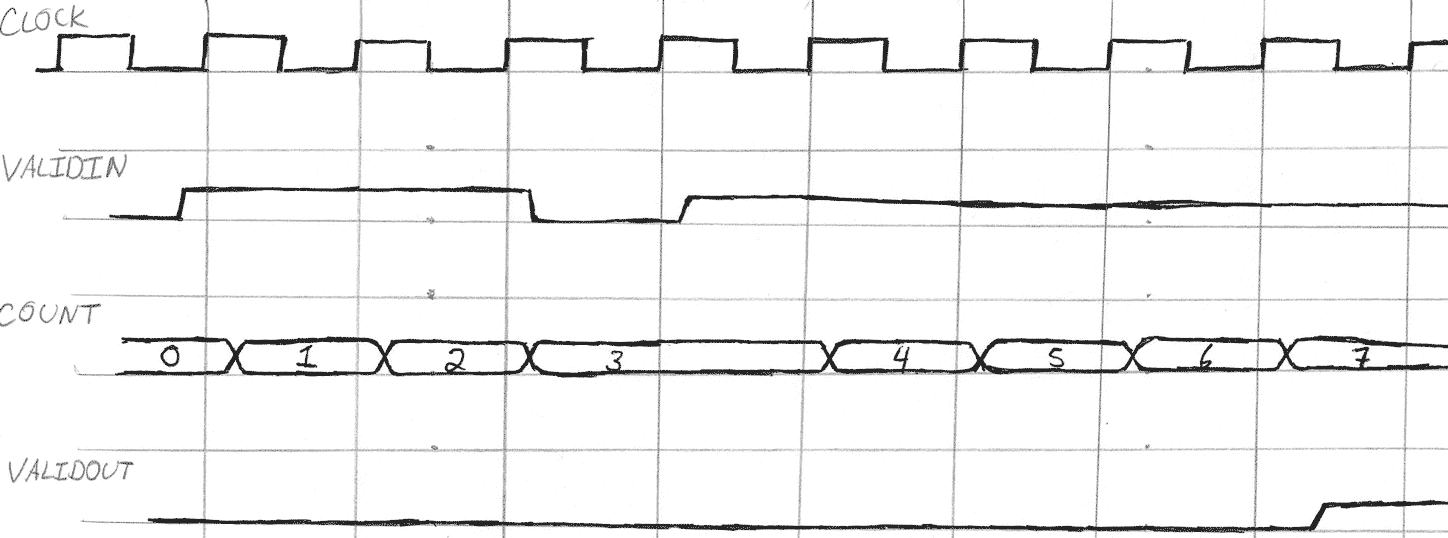
\includegraphics[width=0.75\textwidth]{processed_image_pngs/timing_1.png}

\paragraph{five\_row\_array.v}
This module does need one control signal, asel. What this signal is used for was discussed in the previous section on this module's datapath, and how this signal is generated was discussed in the previous section on five\_by\_five\_window control signals. This module also does not generate any control signals. It does have a simple counter to determine if the pipeline has filled up enough so that the output is valid. This counter will increment as long as there is a valid input, and the count is less than 3*width, where width is the number of pixels in a row (including blanking). Once the count has reached 3*width, the counter will stop incrementing unless the module is reset. The output of the module is invalid if the counter is less than 3*width, or the input is not valid. This also means that an invalid input will stall this module.

\paragraph{y\_window.v}
This module does need one control signal, hsel. What this signal is used for was 
discussed in the previous section on this module’s datapath, and how this 
signal is generated was discussed in the previous section on five\_by\_five\_window 
control signals. This module also does not generate any control signals. It does 
have a simple counter to determine if the pipeline has filled up enough so that 
the output is valid. This counter will increment as long as there is a valid 
input, and the count is less than 5, where width is the number of pixels in 
a row (including blanking). Once the count has reached 5, the counter will stop 
incrementing unless the module is reset. The output of the module is invalid if 
the counter is less than 5, or the input is not valid. This also means that an 
invalid input will stall this module. A timing diagram demonstrating the 
relationship between validin, the counter, and validout is below: 

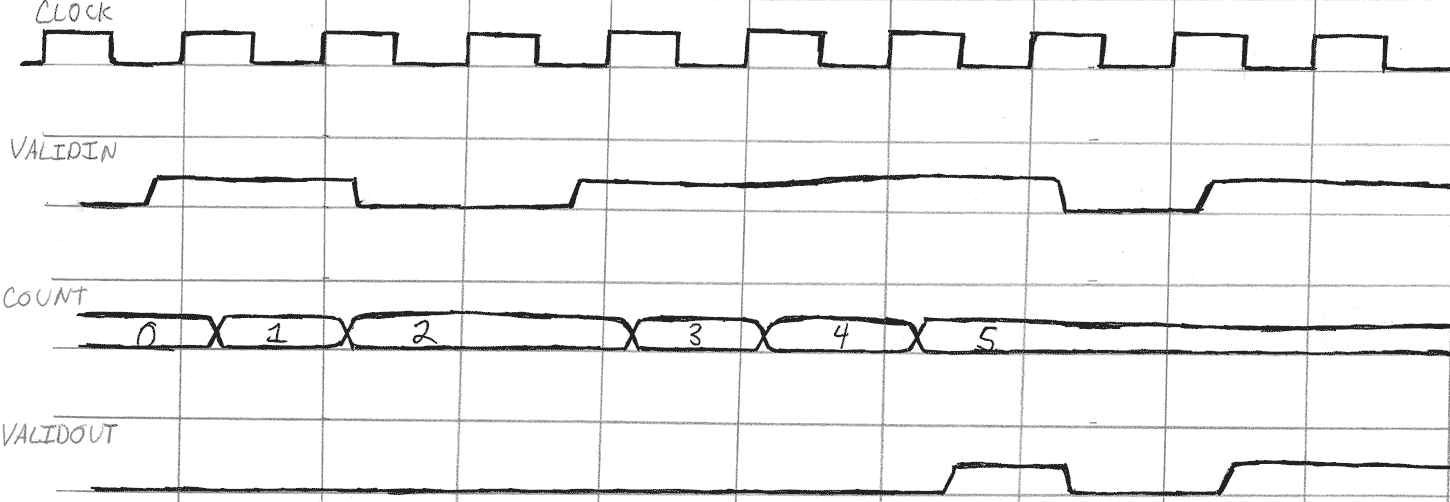
\includegraphics[width=0.75\textwidth]{processed_image_pngs/timing_2.png}

\paragraph{Downsampler.v, Downsampler4x.v}
This module contains various control signals, all of which are driven by either
a modulo or equality computation on a set of counters. These counters naturally
represent our row number and column number in the frame currently being downsampled.
These counters assume that the first valid we recieve is the first valid pixel in a 
frame. The counters then increment as we would expect when receiving a stream of pixels - 
the column (horizontal) counter increments every cycle where valid is asserted, 
while the row (vertical) counter increments every cycle where the column counter
has reached its maximum value (the width of the image minus one). Based on these
values, the Downsampler generates what is effectively a control signal for the
rest of the pipeline, its ``validout'' signal. For ease of reading, the table
below presents the various computations done on the counters to genrate control / 
intermediate signals in the downsampler. The labels presented correspond with
those in the detailed downsampler block diagram shown earlier.

%\begin{wraptable}{r}{10cm}
\begin{figure}
    \begingroup
    \tiny

\caption{ Downsampler (2x) Control / Intermediate Signal Summary } \label{wrap-tab:2}
\noindent \begin{tabular}{ c | c } \toprule
Signal & Boolean Expression \\\toprule
% [todo] - fix the actual numbers
blankingregionin & colcounter $>$ 799 OR rowcounter $>$ 599 \\
rowcounter reset & colcounter == 839 AND rowcounter == 639 \\
colcounter reset & colcounter == 839 \\
rowcounterCE & colcounter == 839 \\
colcounterCE & blankingregionin OR valid \\
validout & (colcounterCE) AND (rowcounter \% 2 == 0) AND (colcounter \% 2 == 0) \\
\end{tabular}
%\end{wraptable}

\endgroup
\end{figure}

\paragraph{Upsampler.v, Upsampler4x.v}
This module contains various control signals, all of which are driven by either
a modulo or equality computation on a set of counters. These counters naturally
represent our row number and column number in the frame currently being upsampled. 
These counters assume that the first valid we receive is the first valid pixel in the 
input frame. The counters then increment as we would expect when receiving a stream
of pixels. In this case, the column (horizontal) counter increments twice for
every valid input that the Upsampler sees, and 800 times after receiving a complete
valid row. The row (vertical) counter always increments immediately after the
cycle during which column counter transitions from (image width - 2) to (image width - 1).
These counters are then used as indicated in the table below to generate control
signals for the rest of the module.

%\begin{wraptable}{r}{10cm}
\begin{figure}
    \begingroup
    \tiny
\caption{ Upsampler (2x) Control / Intermediate Signal Summary } \label{wrap-tab:3}
\noindent \begin{tabular}{ c | c } \toprule
Signal & Boolean Expression \\\toprule
rmod4 & rowcounter \% 4 != 0 \\
cmod4 & colcounter \% 4 == 3 \\
fifo\_read & cmod4 AND (NOT rmod4) \\
validout & rmod4 AND valid \\
rowcounter reset & colcounter == 799 AND rowcounter == 599 \\
colcounter reset & validout AND colcounter == 799 \\
rowcounter CE & prev\_colcount == 798 AND colcount == 799 \\
colcounter CE & validout \\
\end{tabular}
%\end{wraptable}

\endgroup
\end{figure}



\paragraph{Image Switching}
When switching inputs into the ImageBufferWriter, timing is critical. If the switch is made at the wrong time, the output might be shifted over, or the swap controller might get stalled. As mentioned in a previous section, GPIO\_DIP[3:8] is the input to a register. The register is then connected to the mechanism that determines which image writes into ImageBufferWriter. All that is needed is a safe time to update that register. The best time to do this is right after the ImageBufferWriter has completed one frame. Once the ImageBufferWriter signals that it is finished, using bg\_done, the swap controller will send bg\_done\_ack. Once that has happened, the ImageBufferReader, responsible for the DVI output, will get a swap signal from the swap controller. After the ImageBufferReader sends a swap\_ack, the swap controller will issue a start signal (bg\_start) to VGA or StaticImage, and wait for start\_ack. StaticImage will return start\_ack one cycle later, but VGA may have a delay (since it will only issue a start\_ack at the end of a frame). The following timing diagram illustrates this process:

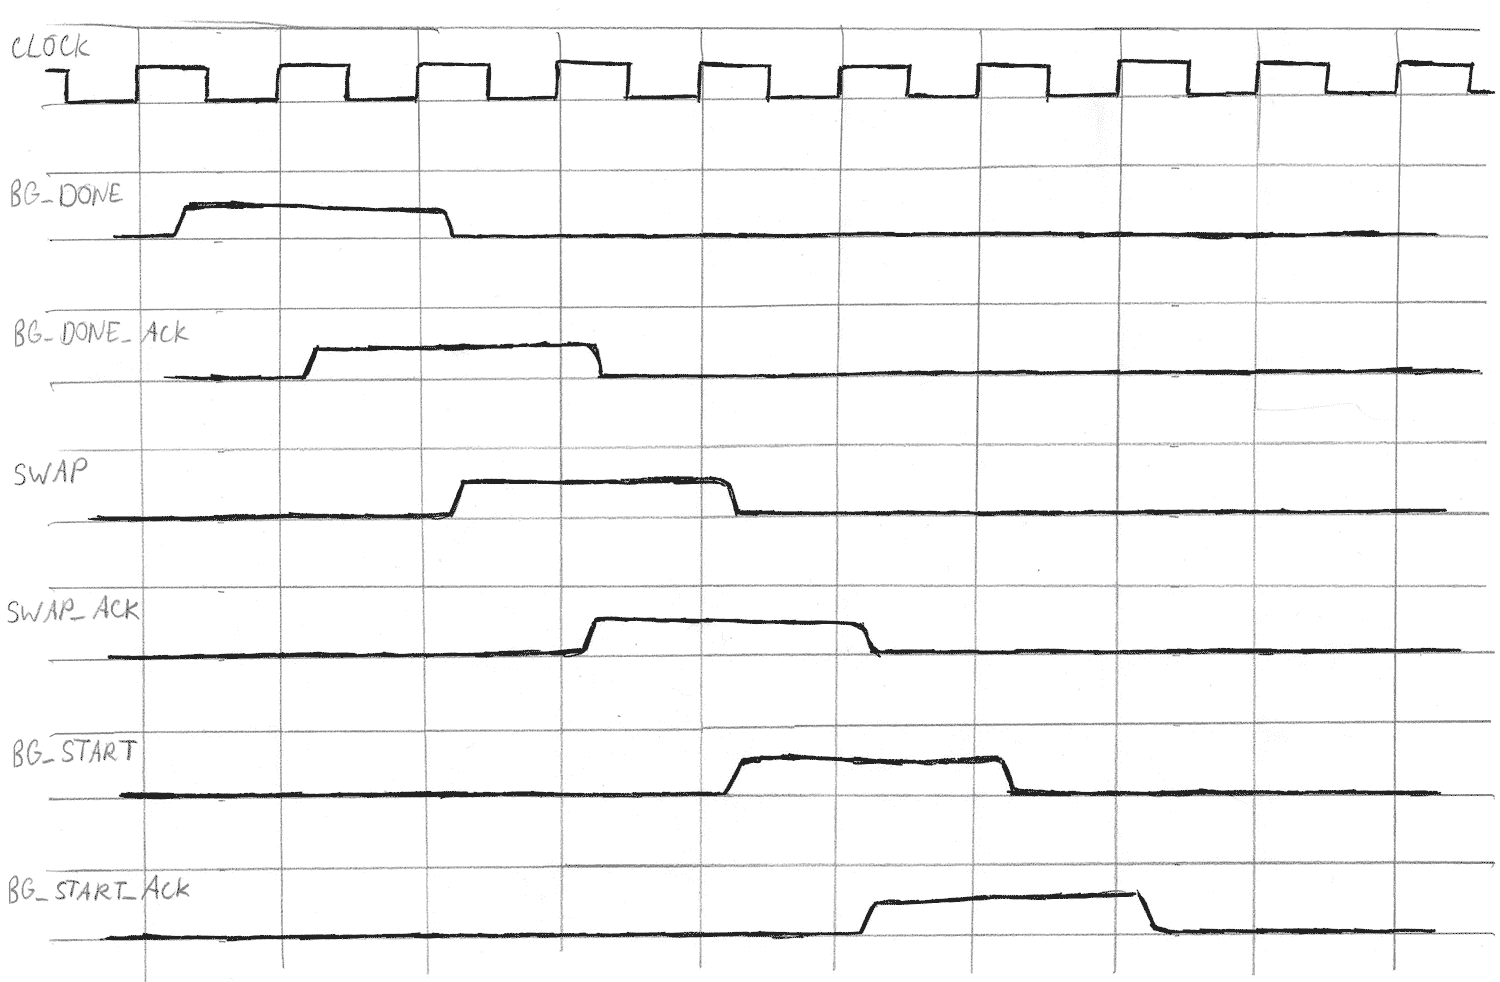
\includegraphics[width=0.75\textwidth]{processed_image_pngs/timing_3.png}

Note that start\_ack may be delayed by one or more cycles if VGA is being used. If this happens, then bg\_start will stay high for the same amount of cycles as the delay.

This gives us plenty of time to check if one of the switches has moved, reset 
the entire pipeline (including each octave, downsampler, and upsampler), and 
then switch the inputs into ImageBufferWriter. We need to reset the pipeline 
because some of the Gaussian filter blocks may still have some non-blanking 
pixels inside, which would be considered valid and would then be pushed into 
ImageBufferWriter. By resetting the pipeline, everything starts over, as if the 
next frame were actually the first frame. We need all of this time because it 
takes more than one clock cycle to reset the FIFOs used in the upsampler and 
downsampler. According to the Xilinx LogiCORE IP FIFO Generator v9.1 User Guide, 
the FIFOs we are using have an asynchronous reset, and it takes three clock 
cycles (write or read) after the asynchronous reset is detected on the rising 
edge read and write clock respectively. Since both the read and write ports 
of all of the FIFOs are on the same clock, that means it will take 3 clock 
cycles before the pipeline is actually ready to receive valid data. From the 
timing diagram above, we see that there will always be enough time to complete 
a reset. Below is an image, taken from the Xilinx LogiCORE IP FIFO Generator 
v9.1 User Guide, which demonstrates the behavior of a FIFO during a reset: 

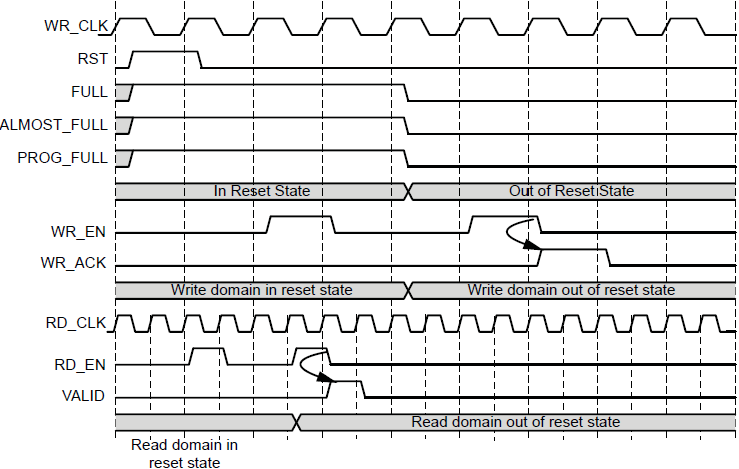
\includegraphics[width=\textwidth]{processed_image_pngs/fifo_timing.png}

\subsubsection{State diagrams and functional timing diagrams}

\section{Design Metrics}

\section{Conclusion}


\end{document}
